%--------------------------------------------
%	PACKAGES AND DOCUMENT CONFIGURATIONS
%--------------------------------------------

\documentclass[11.5pt]{article}
\usepackage{fancyhdr}
\usepackage{gensymb}
\usepackage[ampersand]{easylist}
\usepackage[a4paper, total={8.5in, 11in}, margin = 0.9in]{geometry}
\usepackage{float}
\usepackage{setspace}
\usepackage{titlesec}
\usepackage[version=3]{mhchem} % Package for chemical equations
\usepackage{siunitx} % The \SI{}{} and \si{} command for SI units
\usepackage{graphicx, epstopdf} % Required for the inclusion of images
\usepackage{natbib} % Required to change bibliography style to APA
\usepackage{amsmath} % Required for some math elements
\usepackage[framed,numbered]{matlab-prettifier}
\usepackage{float}
\usepackage{multirow}

\usepackage[utf8]{inputenc}
\usepackage[english]{babel}
\linespread{1.6}

\setlength\parindent{0pt} % Removes all indentation from paragraphs
\renewcommand{\labelenumi}{\alph{enumi}.} % Make numbering in the enumerate environment by letter rather than number 
\setcitestyle{square}


%----------------------------------------------
%	DOCUMENT INFORMATION
%----------------------------------------------
\title{ \textbf{Intelligent Multimodal Prosthetic Hand}}


\author{
	\begin{tabular}{r l l}
	    Adesh Kadambi \\
	    Naseem Alsadi \\
        Nicholas Alfano \\
        Whitney Chu \\\\
	\end{tabular}
	\\
}

\date{Saturday, April 11^{th}, 2020}



\begin{document}


\begin{titlepage}
    \centering
    \maketitle
    \thispagestyle{empty}
\end{titlepage}

\pagebreak



\newpage
\thispagestyle{empty}
\textbf{Executive Summary}
\\\\
This final report presents the final design of the multimodal prosthetic hand that incorporates fully distributed tactile sensing, machine learning, and computer vision techniques. The prosthetics industry is very complex, and our project aims to design a prosthetic hand that can perform human-like tasks with ideal force and precision. This report includes the problem statement, project scope, objectives, societal impacts, constraints, criteria, assumptions, and functional requirements. It also provides background information on current prosthetic hands in the market and a variety of integration techniques. Since the team was able to complete a total of three prototypes, these prototypes are explained in further detail regarding the hardware and software architecture, along with the testing and validation. A cost evaluation has been conducted based on the final prototype that has been designed and created. The team was able to accomplish a majority of the objectives, however, due to the circumstances with COVID-19, limitations were provided. With this, the team determined a variety of future works to finish and improve the project.

\newpage
\thispagestyle{empty}
\tableofcontents
\newpage
\listoffigures
\listoftables
%\lstlistoflistings

\newpage
\pagenumbering{arabic}
\doublespacing

\section{Introduction}

\subsection{Problem Statement}

At its current state, the field of robotics is expanding from its predominant usage in fixed environments like factories or workshops to include more complex environments like homes, offices, and hospitals. This shift in usage comes with a demand for intelligent robots that can interact with humans and be able to perform increasingly human-like manipulation tasks, all while simultaneously sensing and reasoning about their environment \cite{Yousef2011-rc}. Particularly in the application of prosthetics, biological systems have always been a source of inspiration for technological advances. The upper extremity is a highly complex limb with neurovascular bundles, lymphatics, muscles, and bones that come together and form a functional appendage to perform our daily activities \cite{Maduri2019-ry}. The presence of prosthetics can help amputees restore function and enable them to perform daily activities unassisted \cite{Su2019-ws}. Due to engineering limitations, however, there have only been elementary successes \cite{Dehghani2010-yz}. A passive prosthesis may significantly impair grasping and object identification functions, whereas more sophisticated active myoelectric hand prostheses capture EMG from residual muscles and are typically noisy \cite{Su2019-ws, Taverne2019-ve}. Therefore, only a limited number of commands can be used for control, restricting the full potential of usage \cite{Taverne2019-ve}.\\ 

The process of performing the final grasp once the hand is pre-shaped ushers a line of research for the development of artificial skin interfaces with fully distributed tactile sensing, machine learning, and computer vision techniques in hopes of providing information about the forces and positions at all points of contact between the robots and the objects they are interacting with \cite{Yousef2011-rc, Schiefer2018-tt}. Our focus is the solution space surrounding the development of an intelligent prosthetic hand that utilizes multimodal sensory input to perform hand pre-shaping and object grasping without any input from the user, aside from their initial approach towards the object.

\subsection{Scope \& Objectives}

This project aims at extending the solution space mentioned above by utilizing a vision-based approach to perform hand pre-shaping during the reaching phase towards an object and using tactile sensing arrays to determine the object's intrinsic properties and perform the final grasp. Therefore, the prosthetic interfacing and socket design required for a comfortable fit is outside the scope of this project.\\

Our primary objectives within the scope of this project include: (1) the mechanical design of a prosthetic hand with grasping capabilities using 3D modelling software, (2) a low-cost working physical prototype of the prosthetic hand with grasping capabilities, (3) an open-source multimodal sensing software solution to differentiate between different grasp types, and (4) producing an object grasping dataset for future lab-use.

\subsection{Societal Impact}

In the United States alone, an estimated 185,000 persons undergo an amputation of an upper or lower limb each year, totalling an estimated 1.6 million across the country today \cite{Ziegler-Graham2008-cx}. This figure will more than double by 2050 due to the ageing population and associated increase in the number of people living with dysvascular conditions, especially diabetes \cite{Ziegler-Graham2008-cx}.\\

The loss of limb interrupts the closed-loop with the brain that takes place through efferent and afferent pathways, responsible for motor control and sensory feedback, respectively \cite{Cordella2016-ny}. Therefore, the amputation of one's hand can significantly affect the capability of performing daily living, working, and social activities autonomously - demanding a complete lifestyle change. \\

Upper limb prostheses fall into two main categories based on their functional capabilities: passive (or cosmetic) prostheses and active prostheses (which include body-powered and externally powered). Current active prosthetic solutions fail to overcome the struggles faced by prosthetic users due to the limitations in the interfaces adopted for controlling the prosthesis and to the lack of force or tactile feedback, thus limiting hand grasp capabilities \cite{Cordella2016-ny}. Tasks involving in-hand object manipulation, the detection of slippage to adjust grip strength, determining grasp type, and differentiating between deformable and non-deformable objects all prove to be challenging to accomplish. By implementing state-of-the-art sensing technologies, the creation of an intelligent prosthetic hand that replicates the function of a biological hand could significantly improve the quality of life for these amputees. In our case specifically, potential benefits include differentiating between deformable and non-deformable objects to switch between a power grasp and a precision grasp to pick up objects faster and more accurately. \\

With the population of those living with the loss of a limb steadily increasing in the coming years, the need to make prosthetic technology more accessible is more significant than ever. Ziegler-Graham et al. discovered profound disparities in limb loss by race and ethnicity, where the underrepresented minority populations in the United States had a 2-3 times higher risk of amputation than non-Hispanic whites. Recent studies suggest that this variation in risk by race and ethnicity may be credited to poverty and differences in access to primary care and preventative services \cite{Ziegler-Graham2008-cx, Hughes2019-hy}. The cost of a commercial body-powered prosthetic hand can range from \$4000 to \$10,000, and the cost of an externally powered prosthetic hand can range from \$25,000 to \$75,000 \cite{Ten_Kate2017-sf}. For those living in poverty, these prosthetic devices are unaffordable. Although cost is not the primary focus of our project, the development of low-cost prostheses can impact a larger population and be more accessible to those in need, thus strengthening our societal impact.

\newpage
\subsection{Constraints, Criteria and Assumptions}
\subsubsection{Constraints and Criteria}

A set of constraints and criteria (Tables \ref{tab:constraints} and \ref{tab:criteria})  were defined by the client to match the needs of potential users. Several assumptions were made to narrow the scope in order to generate a feasible prototype within the 12-week deadline. However, due to school closures and social distancing practices being mandated as a result of COVID-19, prototyping was discontinued on March 12, 2020.

\begin{table}[H]
\centering
\caption{Project Constraints}
\vspace{3mm}
\begin{tabular}{|>{\arraybackslash}m{7.5cm}|>{\arraybackslash}m{7.5cm}|}
\hline
    \multicolumn{1}{|c|}{Constraint}  & \multicolumn{1}{c|}{Description} \\ \hline
      \textbf{Cost of goods limited to \$450} & With funding and components provided by the University of Guelph and the Robotics Institute lab, a budget of \$450 worth of raw material, as well as hardware, has been put in place. \\\hline
    
    \textbf{Maximum weight of 0.65 kilograms} & Being a daily item worn on an individual in needs arm, a maximum weight of 0.65kg has been put in place. Average robotic prosthetics in the industry weigh from 0.4kg to 1.27kg.  \\\hline
    
    \textbf{Battery life of at least 24 hours} & With the arm being an essential item to those who lack a limb, the need for frequent charging is not acceptable. The product needs to achieve a battery life that will get the user through a full 24-hour day on a single charge. \\\hline
    
    \textbf{Battery must charge fully overnight (6 hours)} & To ensure accessible use it is required that the device obtains a full charge in a maximum six-hour period which is roughly overnight.\\\hline
    
    
     \textbf{Opening span of the gripper must be a minimum of 6cm} & Grasping items 6cm or less allows the user to interact with a large majority of daily objects. \\\hline  
    
\end{tabular}
\label{tab:constraints}
\end{table}

\begin{table}[H]
\centering
\caption{Project Criteria}
\vspace{3mm}
\begin{tabular}{|>{\arraybackslash}m{7.5cm}|>{\arraybackslash}m{7.5cm}|}
\hline
    \multicolumn{1}{|c|}{Criteria}  & \multicolumn{1}{c|}{Description} \\ \hline
    
    \textbf{Minimize the cost of goods used for the prototype} & The prosthetic cost must be minimized in order to increase cost efficiency. Furthermore, remaining at a minimized price point allows for no overage of provided funding.\\\hline
    
    \textbf{The weight of the prosthetic is to be minimized.} & The prosthetic is supposed to be an extension of one’s limb. Making the product as light as possible ensures that the user would not feel encumbered by the product while in use.  \\\hline
    
     \textbf{Battery life of the prosthetics is to be maximized} & To warrant the prosthetic’s use, the user must feel as though they can rely on the product to last a realistic time frame. Otherwise, one may be averse to utilizing the product due to an apparent lack of reliability. \\\hline
    
    \textbf{Aesthetics} & To ensure the use of the prosthetic it must resemble that of a real hand. Moreover, functionality is integral as it must allow the user to engage with their physical environment by grasping objects.\\\hline
    
\end{tabular}
\label{tab:criteria}
\end{table}

\newpage
\subsubsection{Assumptions}

Below are the assumptions made to proceed with this project:

\begin{itemize}
    \item Only two fingers are required to grasp all objects.
    \item The user will be capable of guiding the hand towards the object. 
    \item It is assumed that the designed prosthetic will fit the user. 
    \item Assume the size of the objects will fit within the hands grasping span.
    \item The user will be competent with respect to charging the device as needed.
\end{itemize}



\subsection{Functional \& Non-Functional Requirements}

\begin{figure}[H]
    \centering
    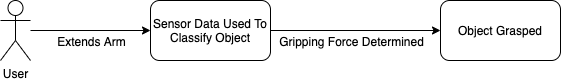
\includegraphics[width=0.8\linewidth]{Circuits/funreq.png}
    \caption{Basic overview of system functionality.}
    \label{fig:funreq}
\end{figure}

\textbf{Functional Requirements}

\begin{itemize}
    \item Hand is pre-shaped to object dimensions via optical input prior to closing.
    \item System can freely open or close to grasp as object.
    \item Upon closing, sensory systems will determine intrinsic object properties.
    \item System will map the object image and tactile input to grasp configuration.
    \item Control system will regulate and maintain grasp using continuously recorded tactile data.
\end{itemize}

\textbf{Non-functional Requirements}

\begin{itemize}
    \item Data collection and streaming meet HIPAA requirements.
    \item Near real-time computational performance for object grasping.
    \item System programming shall not use deprecated code.
    \item Open-source software solution for better maintainability.
    \item Device is portable and software is cross-platform.
\end{itemize}

\newpage
\section{Literature Review}

\subsection{Manufacturing}

Over the past five years, there has been significant growth in the use of 3D printing technology, including the printing of upper limb prostheses. 3D printing presents a variety of advantages over traditional manufacturing processes, including rapid design improvements, having the design freedom to include complex geometries, and operating at a fraction of the cost. The print specifications of several hand prostheses in scientific literature reveal production costs of between \$300 and \$500, enabling access to all populations and demographics \cite{Ten_Kate2017-sf}.

\subsection{Tactile Sensing}

Tactile sensing, in the robotics field, is defined as the continuous sensing of variable contact forces \cite{Pennywitt1986-ww}. Using this knowledge can significantly improve the performance and confidence of object classification, contact configuration, and grasp stability \cite{Schiefer2018-tt}. Much like the human hand's somatosensory feedback mechanism, these advanced tactile sensors are becoming increasingly pivotal in facilitating safe and dexterous interaction between robots and their environments \cite{Schiefer2018-tt, Charalambides2017-vy}. \\ 

From a biological perspective, tactile receptors are grouped in clusters on the skin around the human body. The actual sense of touch involves different nerve types and sensing subsystems to relay a whole-body experience \cite{Dargahi2004-tv}. The somatosensory system, in particular, deals with the spatiotemporal perception of external stimuli through mechanoreceptors, thermoreceptors, and nociceptors \cite{Dargahi2004-tv}. These receptors are responsible for the determination of pressure, vibration, temperature, and pain. Using these responses, the human hand can perform tactile object recognition. By equipping a prosthetic hand with multi-modal tactile sensing arrays, including sensors for static pressure, dynamic pressure, thermal, and proximity sensors, we can mimic this biological intelligence \cite{Dargahi2004-tv}. \\

Artificial tactile sensors contain pressure profile sensing arrays, force-torque sensors, and dynamic tactile sensors. Depending on the capabilities of the sensor array, one can determine contact locations, reconstruct and recognize object shape, and even measure the various contact forces \cite{Stillfried2014-to}. Current applications of these sensors include sensing technologies for robot hands, minimally invasive or robotic surgery, biomedical applications, and slip detection in hand prostheses, to name a few. Several design considerations are surrounding the selection criteria of these tactile sensors (Table \ref{table:design}).

\begin{table}[H]
    \centering
    \caption{Design consideration pros and cons.}
    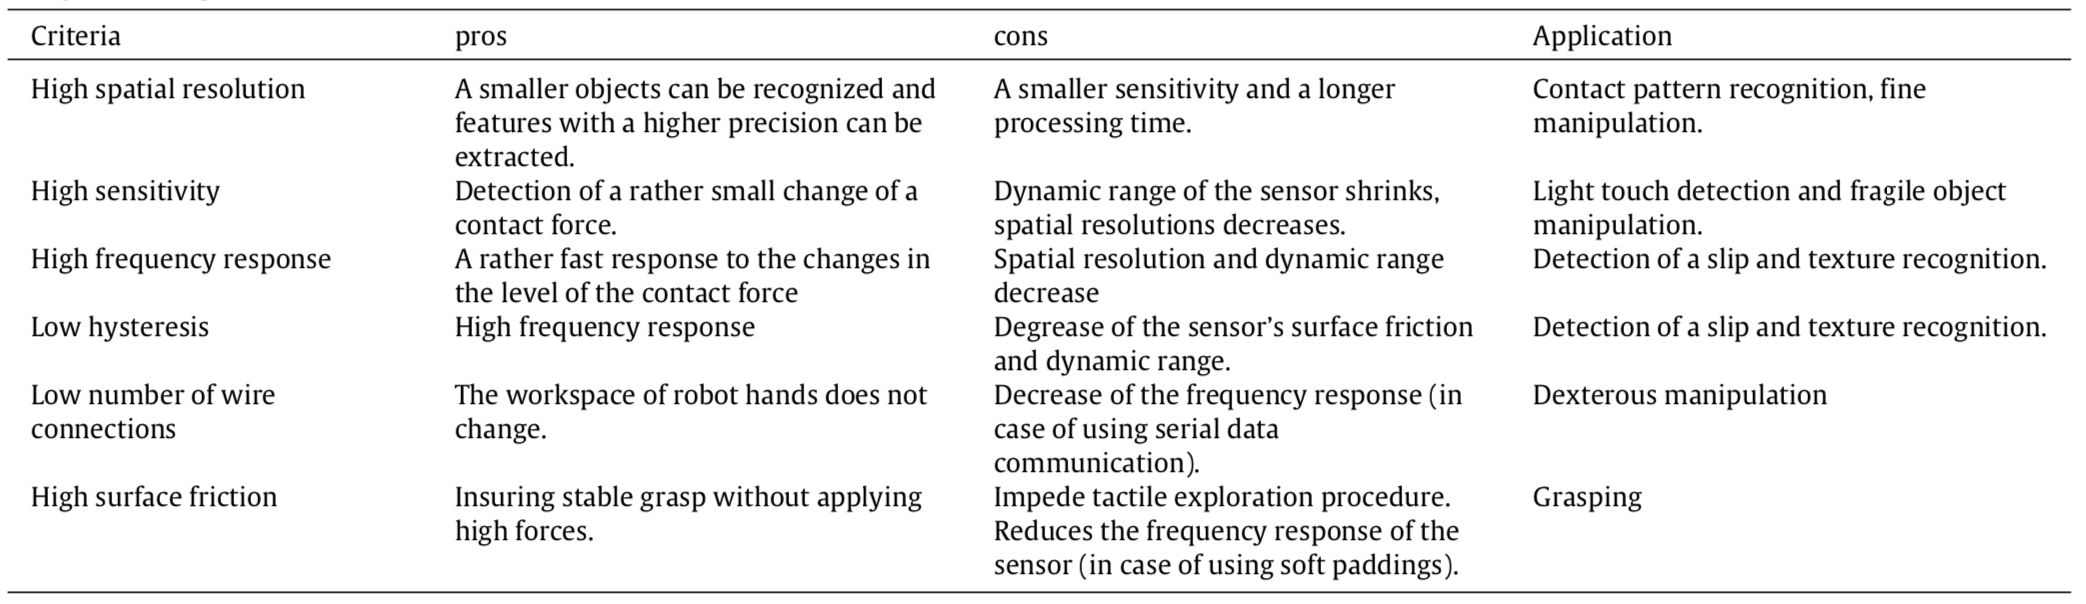
\includegraphics[width=1.0\linewidth]{assets/designprocon.png}
    \label{table:design}
\end{table}

\subsection{Data-driven Grasping}

\textit{Li et al.} present a cross-modal prediction system between vision and touch with the goals of generating tactile results from image input and vice versa. To investigate the connections between touch and vision, they introduced two cross-modal prediction tasks: (1) synthesizing plausible temporal tactile signals from vision inputs, and (2) predicting which object and which object part is being touched directly from the tactile data \cite{Li2019-eu}. To accomplish this, they use the pix2pix method, a generative adversarial network (GAN) framework for image-to-image translation (Figure \ref{fig:li}). In the context of cross-modal prediction, the generator \texttt{G} takes either a vision or tactile image \texttt{x} as an input to produce an output image in the other domain with \texttt{y=G(x)}. The difficulty arises when attempting to solve the extrapolation problem of localizing the location of the touch and then inferring the material and geometry of the touched region. Although \textit{Li et al.}'s findings may help object recognition and grasp in low environment settings, the time commitment required to build the dataset and train a GAN makes this option unfeasible for a 9-week project.

\begin{figure}[H]
    \centering
    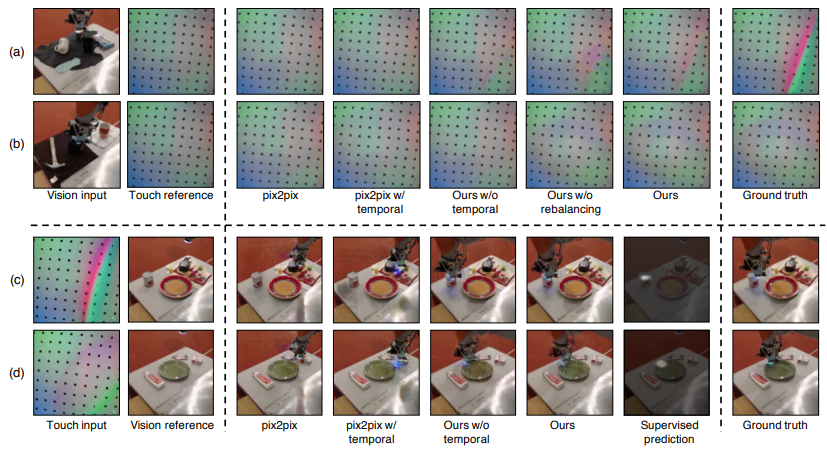
\includegraphics[width=0.88\linewidth]{assets/li.png}
    \caption{Example cross-modal prediction results. (a) and (b) show two examples of vision to touch prediction by our model and baselines. (c) and (d) show the touch to vision direction.}
    \label{fig:li}
\end{figure}

\newpage

\textit{Calandra et al.} propose an end-to-end action-conditional model that learns re-grasping policies from raw visuotactile data. Their deep, multimodal CNN predicts the outcome of a candidate grasp adjustment as a Markov decision process and then executes a grasp by iteratively selecting the most promising actions (Figure \ref{fig:calandra}). Their approach eliminates the need for calibration of the tactile sensors or any analytical modeling of contact forces, thus significantly reducing the engineering effort and making it an appealing avenue for us to pursue. The visuotactile model identified the importance of modulating the amount of force \texttt{F} applied at the fingers for the grasp outcome \cite{Calandra2018-zy}. 

\begin{figure}[H]
    \centering
    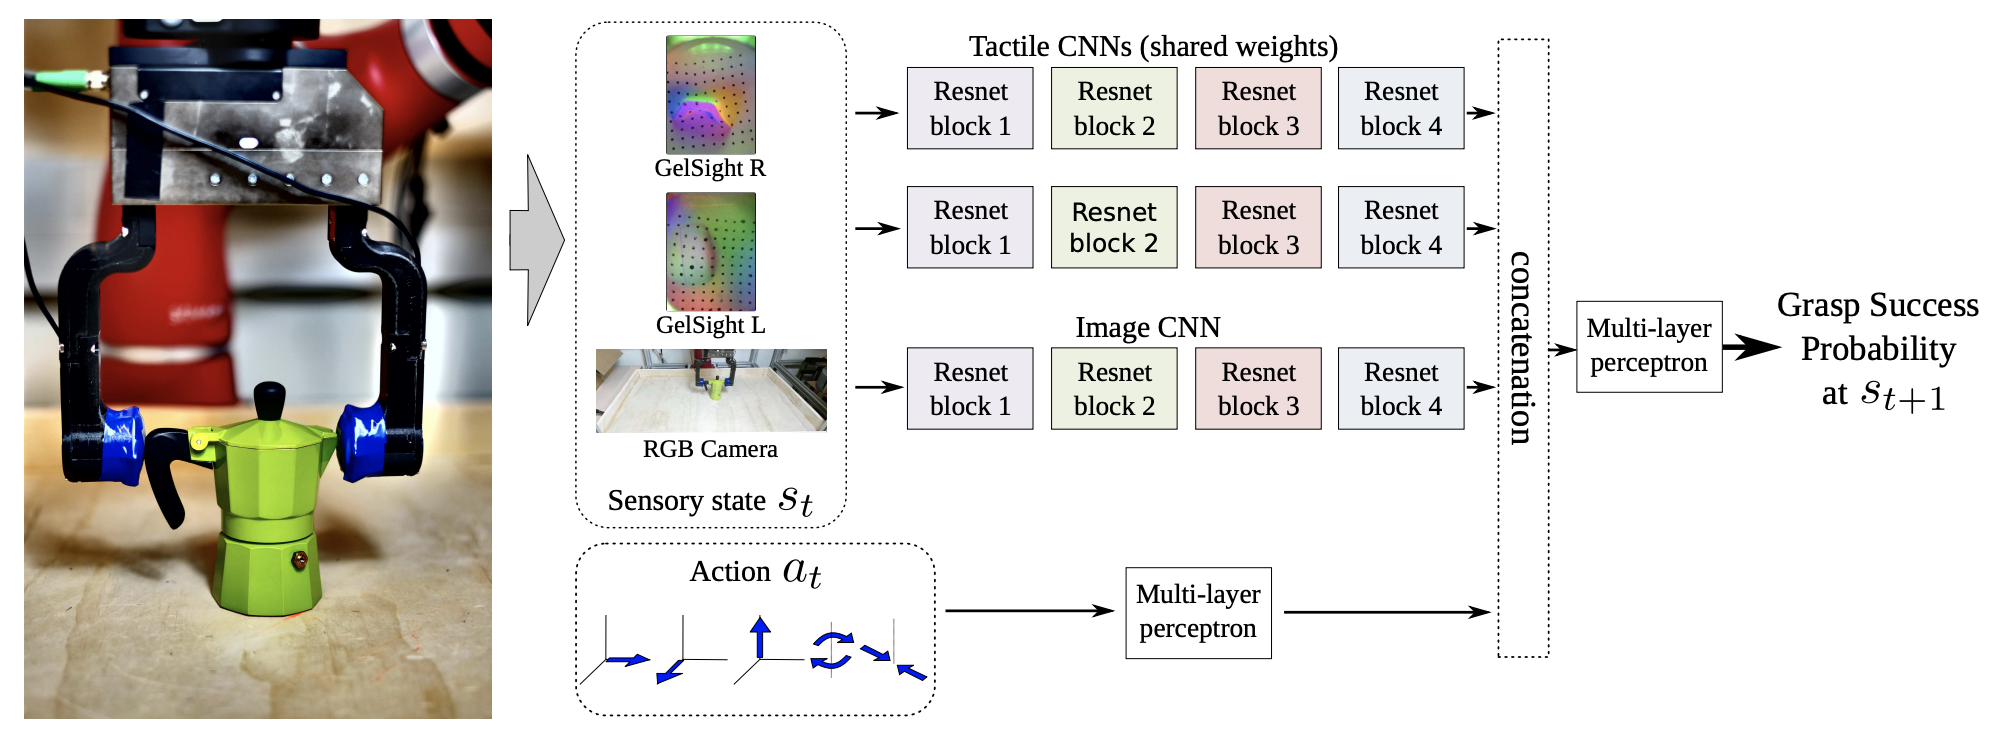
\includegraphics[width=0.95\linewidth]{assets/calandra.png}
    \caption{Action-conditioned visuotactile model network architecture.}
    \label{fig:calandra}
\end{figure}

Objects held close to their top might slip away under even small perturbations, whereas objects grasped below the center-of-mass might be unstable and rotate around the contact, increasing the chance of slippage. However, the action-conditional grasp outcome prediction model did not seem to learn any relevant correlation surrounding center-of-mass, a limitation that arose due to their focus on coarse actions. A model using fine-grained actions could more delicately manipulate the object before the grasp and potentially react to slippage during the lift-off, similar to Ian's work.  Additionally, the action-conditioned model only makes single-step predictions and does not perform information-gathering actions, presenting a novel avenue for our project scope \cite{Calandra2018-zy}.\\

The similarity between both of these studies is the use of GelSight optical sensors. Although they produce images in impressive spatial resolution, \textit{Takahashi et al.} claim they are easily damaged during contact and thus require frequent maintenance in contact-rich manipulation tasks such as grasping. As a result, they opt for the commercialized uSkin sensors that utilize magnets to measure the deformation of silicon during contact by monitoring changes to the magnetic fields \cite{Takahashi2018-yg}. Under the assumption that both the GelSight and uSkin sensors are exorbitantly priced, we propose the use of signal processing techniques to convert the integer array outputs from the tactile sensors to an image, potentially yielding similar findings to those found in \textit{Calandra et al}.\\

\newpage

An amalgamation of variant modalities is a challenging task when dealing with robot control. Deep reinforcement learning has proven successful in dealing with high-dimensional inputs. However, the implementation of deep reinforcement learning in real robots is burdensome due to considerable sample complexity. \textit{Lee et al.} propose a novel self-supervision model, grounded in the ability to learn multimodal representations of peripheral sensory inputs. The core sensory inputs utilized in this study were vision, touch, and proprioception. Implementation of a unique multimodal fusion module, employing variant encoding and decoding architectures, allowed for optimal sensory input utilization \cite{Lee2018-gm}. The collaboration of multilayer perceptrons and convolutional neural networks to encode and decode variant input sources provided a reliable and accurate backbone to the model (Figure \ref{fig:lee}).

\begin{figure}[H]
    \centering
    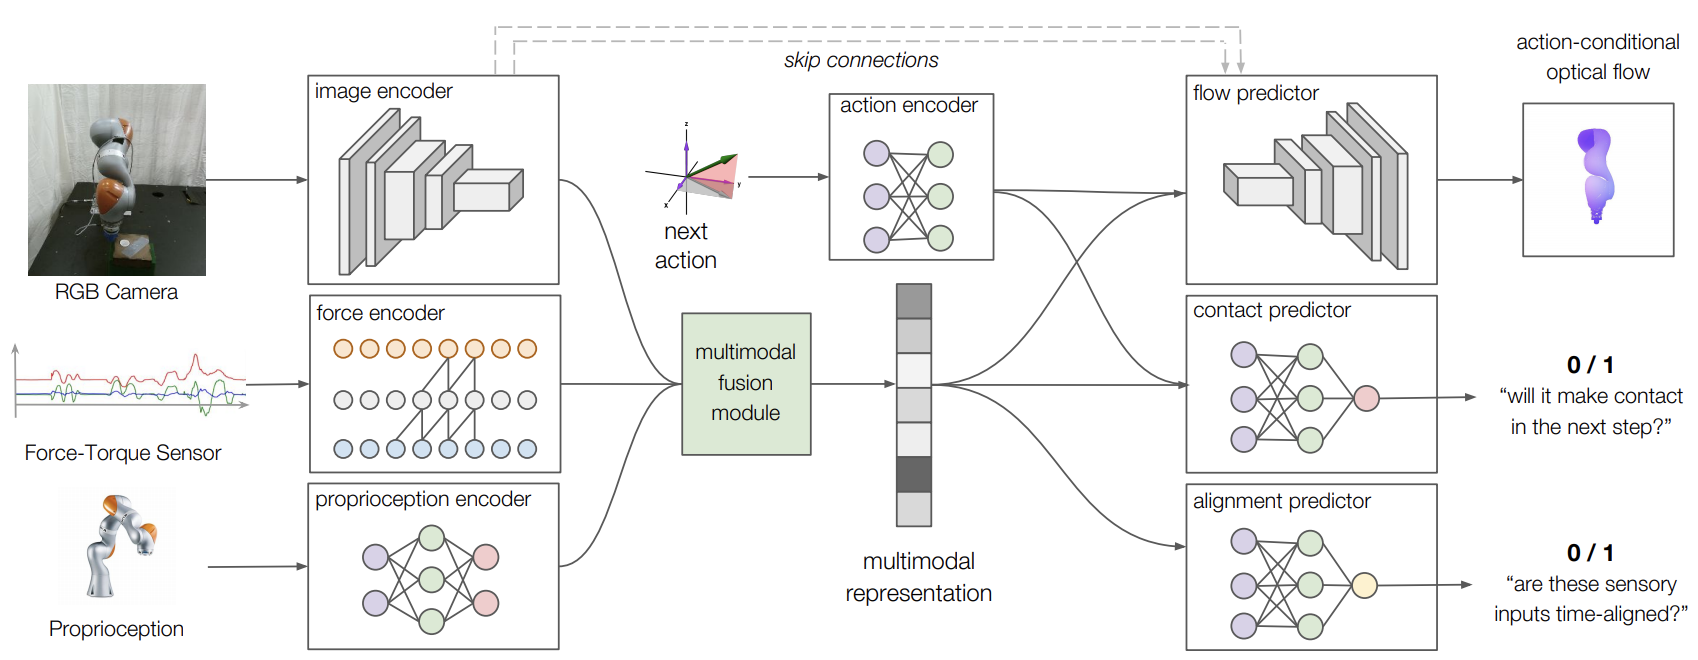
\includegraphics[width=0.88\linewidth]{assets/lee.png}
    \caption{Action-conditional neural network architecture for multimodal representation learning with self-supervision. The network takes data from three different sensors as input: RGB images, F/T readings over a 32ms window, and end-effector position and velocity. It encodes and fuses this data into a multimodal representation based on which controllers for contact-rich manipulation can be learned.}
    \label{fig:lee}
\end{figure}


\newpage
\section{Detailed Design}
\subsection{Overview}
The system is equipped with peripheral sensors to accomplish our primary objective of developing an intelligent hand with the ability to grasp objects by autonomously regulating grasping force (Figure \ref{fig:HGI}). These sensors ensure that the system is capable of interacting with its environment by receiving information from its surroundings and proactively maneuvering its way through space. The design necessitates a hand with a dynamic gripping mechanism. In order to regulate the gripping force, the motor driving the gripping must allow a wide range of functionality, ensuring that the gripping force can be selected. Furthermore, the design needs a control unit that can receive input from the selected peripheral sensors, as well as deliver an output signal to the gripping mechanism. The control unit must be physically present. However, it must be able to host the software side of the design. The software will read the input provided by the peripheral sensors and ultimately provide a respective motor torque value. The software output is sent to the respective motor, which will then drive the gripping mechanism per the selected value.

\begin{figure}[H]
    \centering
    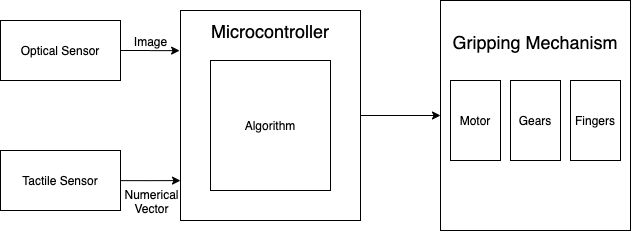
\includegraphics[width=0.8\textwidth]{Circuits/Hardglow.png}
    \caption{System overview.}
    \label{fig:HGI}
\end{figure}
 
\subsection{Software Architecture}
The proposed model architecture can be dichotomized into three separate phases (Figure \ref{fig:overall}). The Deep Learning Phase and Motor Torque Calculation Phase are the highest ordered stages that consistently execute throughout run time.

\begin{figure}[H]
    \centering
    
\includegraphics[width=1.0\textwidth]{assets/Model.png}
    \caption{Model architecture is split into three phases: Sensory, Deep Learning, and Motor Torque Calculation. Optical and tactile inputs are fed into seperate pipelines before concatenating and classifying grasp type. A power grasp closes the fingers at full power and a precision grasp determines motor torque based on tactile sensor feedback control system.}
    \label{fig:overall}
\end{figure}

\subsubsection{Deep Learning Phase}

The Deep Learning Phase deals with a binomial classification problem, namely classifying between a power or precision grasp. The input to this phase is the visual perception unit, delivering an optical data stream of the external world, and the tactile sensing unit, delivering a somatic pressure based data flow. The optical pipeline feeds data into a Convolutional Neural Network (CNN) and the tactile sensing pipeline feeds into a Multi-Layer Perceptron (MLP). The outputs of the CNN and MLP are concatenated and directed towards a final MLP. The Deep Learning Phase is summarized in Figure \ref{fig:cumflow}, while sub-components are explained below.

\begin{figure}[H]
    \centering
    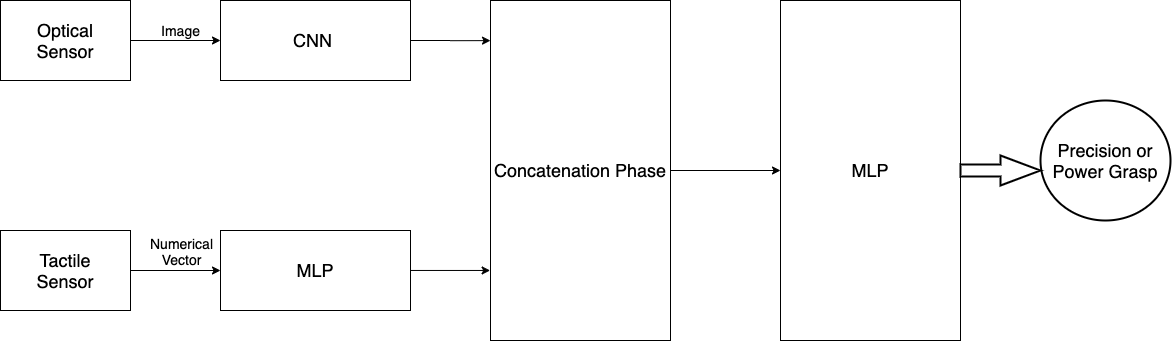
\includegraphics[width=0.95\linewidth]{assets/CumFlow.png}
     \caption{Deep Learning Phase Diagram}
    \label{fig:cumflow}
\end{figure}

A CNN architecture is a class of deep neural networks commonly utilized in image analysis and classification. A CNN is primarily composed of convolution layers and pooling layers. The convolution layers use filtering to extract features from a raw image. Pooling layers reduce the dimensions of the feature map, therein scaling down the number of parameters and minimizing computation. CNN’s contain the ability to learn feature representation from raw data autonomously. This allows the model to learn abstract features from a provided set of training data and apply feature representation in classifying testing data. Figure \ref{fig:CNND} displays an overview of the CNN procedure.

\begin{figure}[H]
    \centering
    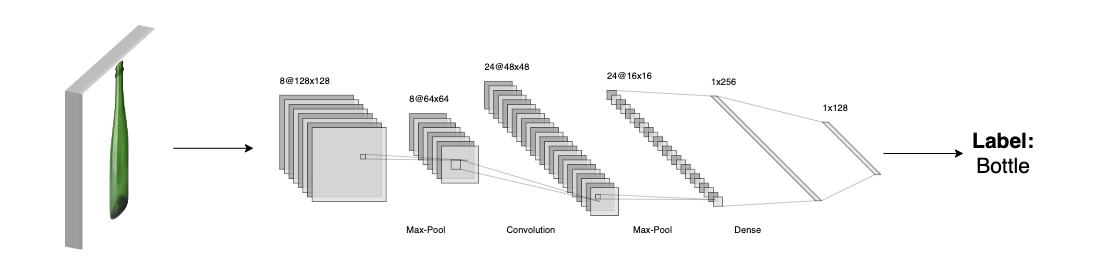
\includegraphics[width=1.02\textwidth]{assets/CNND.png}
    \caption{Convolutional Neural Network Diagram}
    \label{fig:CNND}
\end{figure}

The CNN will process the visual input and learn feature representations that will lead to precise object classification. To achieve an accurate model, the model was trained on visual data specific to the object space, as well as general data to ensure model flexibility. Figure \ref{fig:WBC} shows an accurate classification of a bottle. The sole use of the CNN ensures that architecture is capable of classifying the object in view, however, object characteristics will largely remain a mystery without the assistance of the tactile sensing pipeline. For instance, the bottle shown in Figure \ref{fig:WBC} was correctly classified, although nothing has been said about the type of bottle it is. The bottle may be made of glass or the liquid inside maybe frozen, therein decreasing deformability. Attempting to train the model to capture these variances will dramatically increase sample complexity, and not accounting for these variances will reduce correct functionality when operating outside of the selected object space.

\begin{figure}[H]
    \centering
    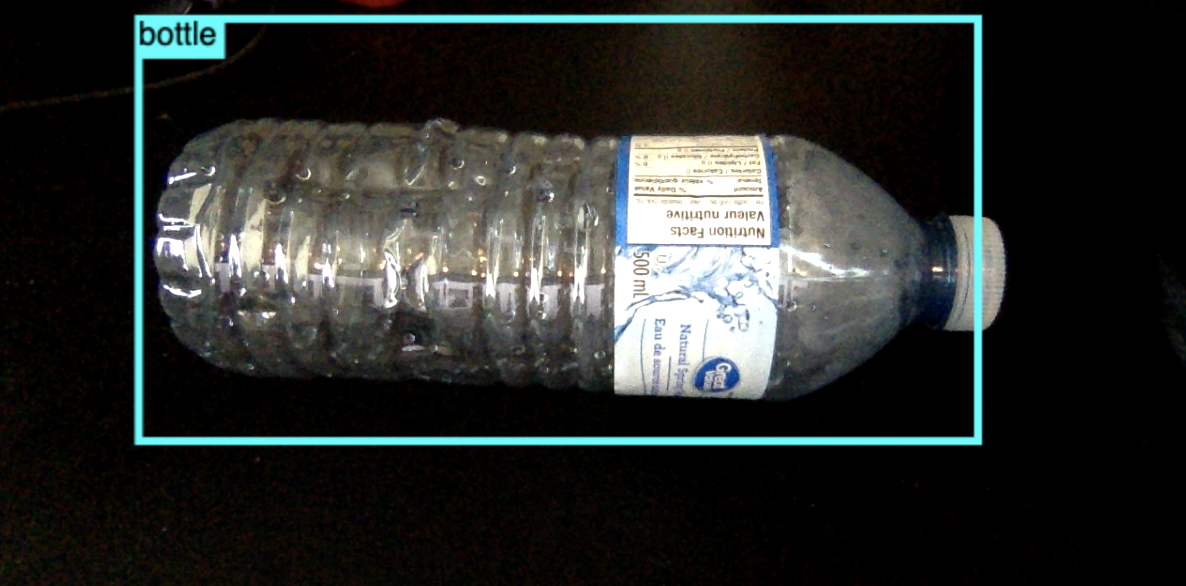
\includegraphics[width=0.6\textwidth]{assets/Bottleclass.png}
    \caption{Real-Time Water Bottle Classification}
    \label{fig:WBC}
\end{figure}

To combat this issue the introduction of the tactile sensing unit was necessary. Information obtained from the use of the tactile sensors flows through the tactile data pipeline. This pipeline feeds raw data into a Multi-Layer Perceptron (MLP). An MLP is a class of feedforward artificial neural networks. It is sub-composed of 3 variant layers, namely, input, hidden and the output layers.  The MLP relies upon an algorithm called backpropagation to learn feature representations.  The output of the MLP is a classification of the characteristics of the object based upon the tactile sensing input data.  Characteristics yielded from the MLP can be grouped under the umbrella term of rigidity characteristics.\\

The MLP and CNN must not be treated as mutually exclusive networks, rather they both assist each other by correctly classifying the targeted object. Without the CNN, the architecture is rather rudimentary and basic. Relying upon only the input from the tactile sensors leaves us only with a close-range analysis of the object, without extracting crucial detail evident when viewing the object as a whole. \\

After the input data has made its way through both the CNN and initial MLP, the outputs of both networks are concatenated. At this stage, the object label and the object characteristics are amalgamated into a singular vector. This allows for the use of a decisive MLP, which reads in the novel vector and decides whether a precision grasp or power grasp is necessary. The Deep Learning Phase concludes when the respective grasp type has been determined, passing on the output to the next phase.

\subsubsection{Motor Torque Calculation Phase}

The exact functionality and procedure of this phase is dependent on the output of the Deep Learning Phase. In essence, there are two mutually exclusive modes of functionality, namely power grasping and precision grasping. The selection of the power grasping mode entails a non-dynamic grasping function, simply closing without restriction to force. The selection of the precision grasping mode necessitates a PID controller with tactile sensing input and motor torque output. The PID controller monitors the process variable meanwhile calculating an error value as the variance between the setpoint and the process variable. The error value is then utilized in the adjusting of the control variable. With regard to this specific application, the tactile sensor data is monitored and compared against a desired tactile sensor data value. The calculated error value is therein used to adjust the motor torque value. \\

Precision grasping presents a greater challenge from the two modes of functionality. A systematic approach was taken to ensure that the dynamic controller consistently interacted with its environment. The procedure followed when precision grasping mode is activated can be seen in Figure \ref{fig:PID}. 

\begin{figure}[H]
    \centering
    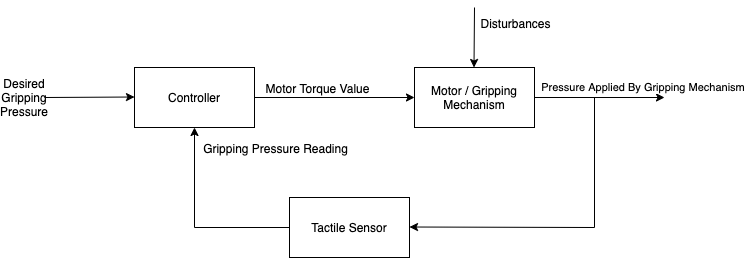
\includegraphics[width=0.955\textwidth]{assets/CSBD.png}
    \caption{Feedback Control System Block Diagram}
    \label{fig:PID}
\end{figure}

The control system seen in Figure \ref{fig:PID} reflects the cumulative system and environment exchange. The system is initialized with a setpoint value, indicating the desired gripping pressure based on the tactile sensory unit. The controller takes in the setpoint value, as well as the current gripping pressure reading from the active tactile sensors, referred to as the process variable. Within the controller, an error value is calculated according to the difference between the setpoint and the process variable. The controller then outputs a unique motor torque value intending to combat the calculated error. The controller output value is dictated towards the motor, which in turn manipulates the gripping strength. 

\newpage
\subsection{Mechanical Design: Prototype One}

The initial plan was to utilize a Fanuc 200id robotic arm to help with testing. With this notion, the first prototype was created to aesthetically resemble a 1 DoF open/close pinch end effector (Figure \ref{fig:hh}). After re-evaluating the time constraint, it was decided that the prototype would be maneuvered by a team member for testing. This resulted in the need for a handle to conveniently grasp to simulate the use of the prosthetic by one who lacks a hand.\\

\begin{figure}[H]
\centering
\begin{subfigure}
  \centering
  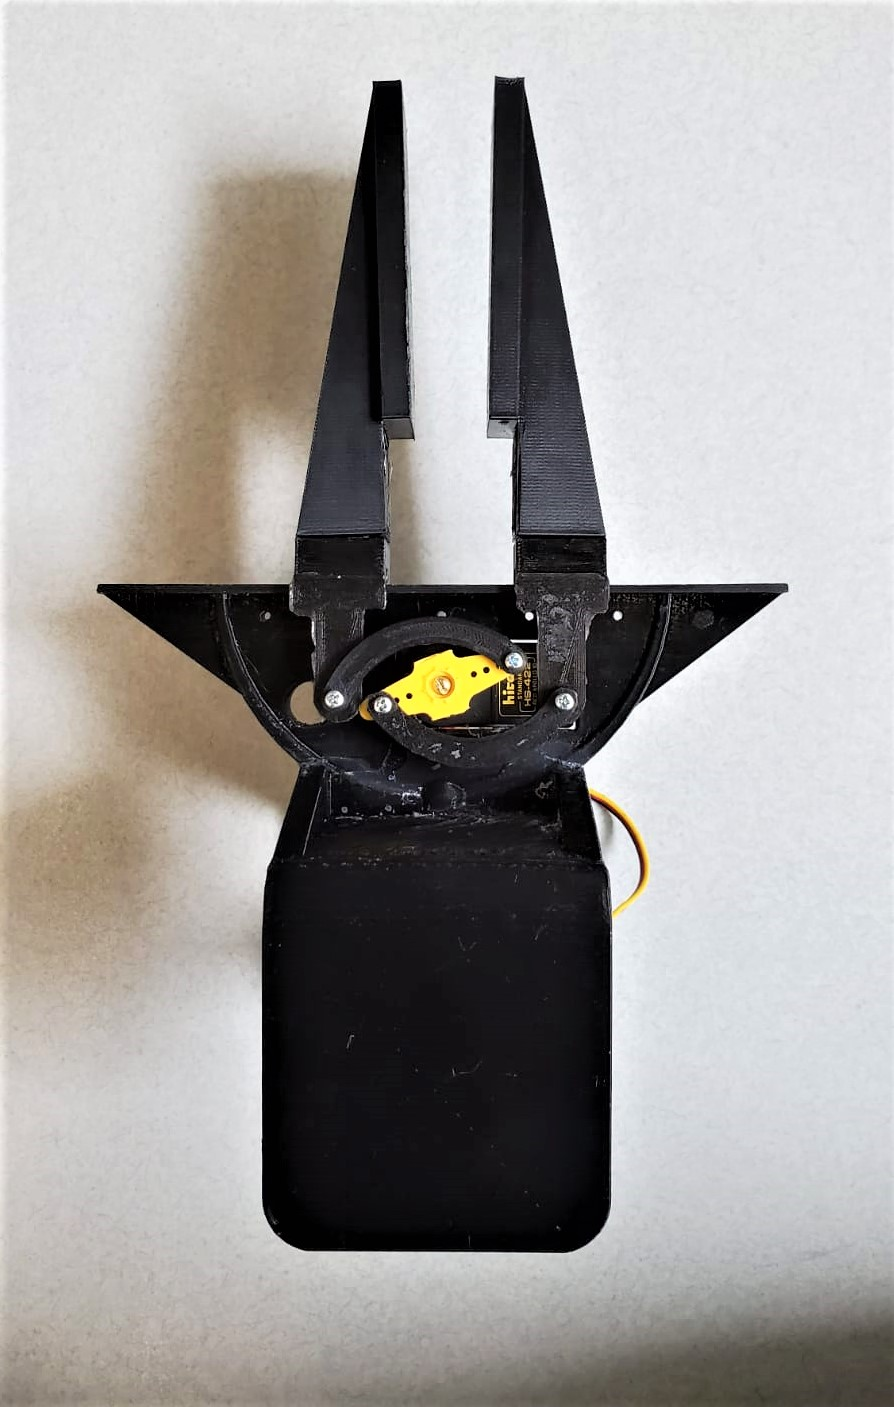
\includegraphics[width=0.25\columnwidth]{2d/WhatsApp Image 2020-02-14 at 2.43.31 PM.jpeg}
  \label{fig:sub1}
\end{subfigure}%
\begin{subfigure}
  \centering
  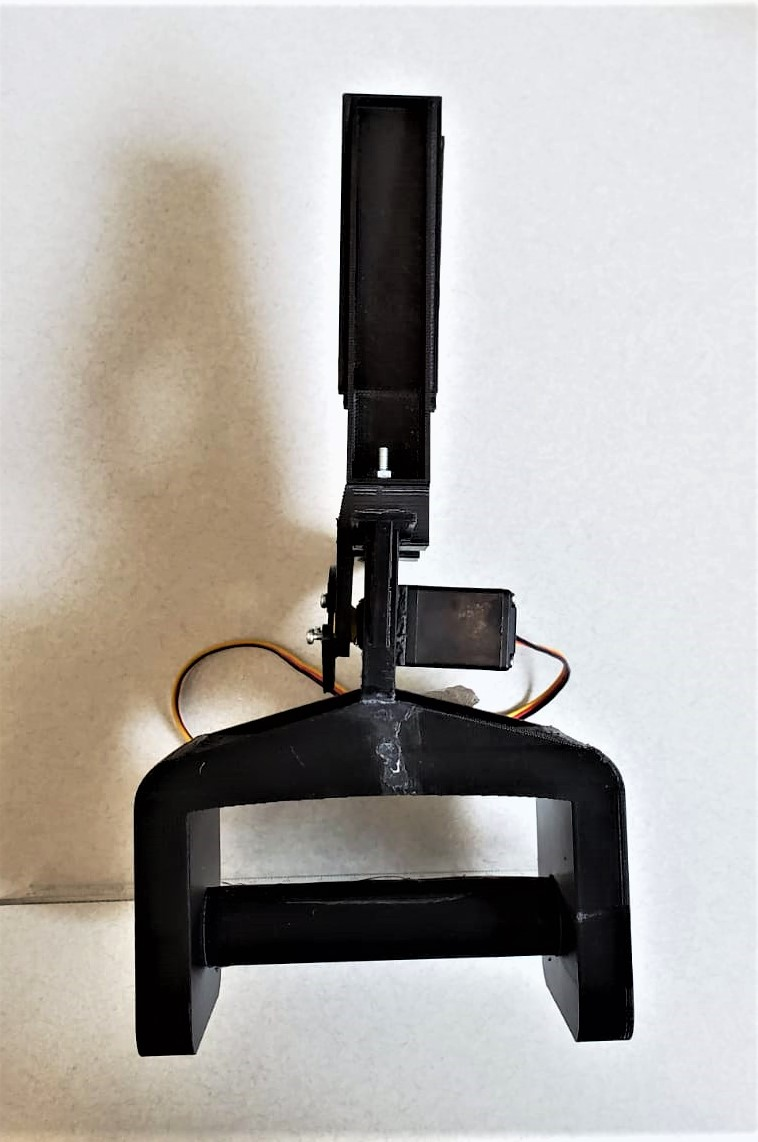
\includegraphics[width=0.263\columnwidth]{2d/WhatsApp Image 2020-02-14 at 2.51.39 PM.jpeg}
  \label{fig:sub2}
\end{subfigure}
\caption{Images of the First 3D-Printed Model}
\label{fig:hh}
\end{figure}

CAD modeling was completed using SolidWorks 2019, and a labeled 3D render of Prototype One can be seen in Figure \ref{fig:de} and Table \ref{tab:se}. Prototype One consisted of a base, exhibiting a 6-inch-long track. Along the track lie two arms that slide along the x-axis of the track to perform a pinch. With 1in x 1in tactile sensors chosen, the two arms were designed with a contact surface to precisely fit the sensory. A HS-422 servo motor was fixed to the centre of the base of the model to open and close the arms. The motor is then connected to two curved brackets, which translates the angle of rotation of the motor to arm locations along the track. This designed mechanism allows the arms to open to a span of 6.5cm. A handle is fixed to the bottom of the model for testing purposes. The 3D printed model and the SolidWorks 3D model renderings can also be seen in Figure \ref{fig:de} and \ref{fig:actual}, respectively. The 2D drawings for prototype one can be found in Appendix A.1.1.

\begin{table}[H]
\centering
\caption{Mechanical Components of Prototype One}
\vspace{3mm}
\begin{tabular}{|>{\arraybackslash}m{3cm}|>{\arraybackslash}m{3cm}|}
\hline
    \multicolumn{1}{|c|}{Number}  & \multicolumn{1}{c|}{Component} \\ \hline
    \textbf{1} & Track/Base \\\hline
    \textbf{2} & Arm  \\\hline
    \textbf{3} & Handle \\\hline
    \textbf{4} & Servo Motor\\\hline
    \textbf{5} & Bracket\\\hline
\end{tabular}
\label{tab:se}
\end{table}

\begin{figure}[H]
    \centering
    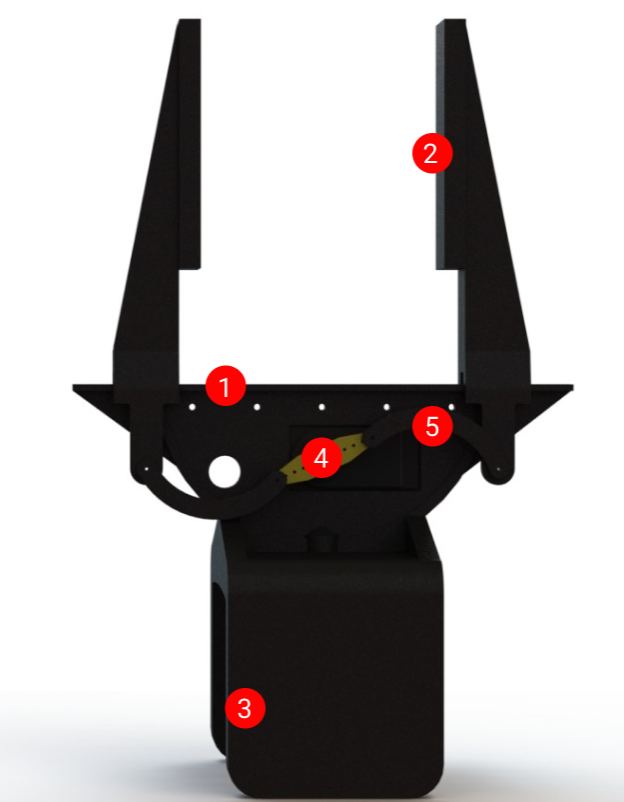
\includegraphics[width=0.35\linewidth]{2d/3DModelsPics/Screenshot (8).png}
    \caption{Prototype One Labeled 3D Model}
    \label{fig:de}
\end{figure}



\begin{figure}[H]
\centering
\begin{subfigure}
  \centering
  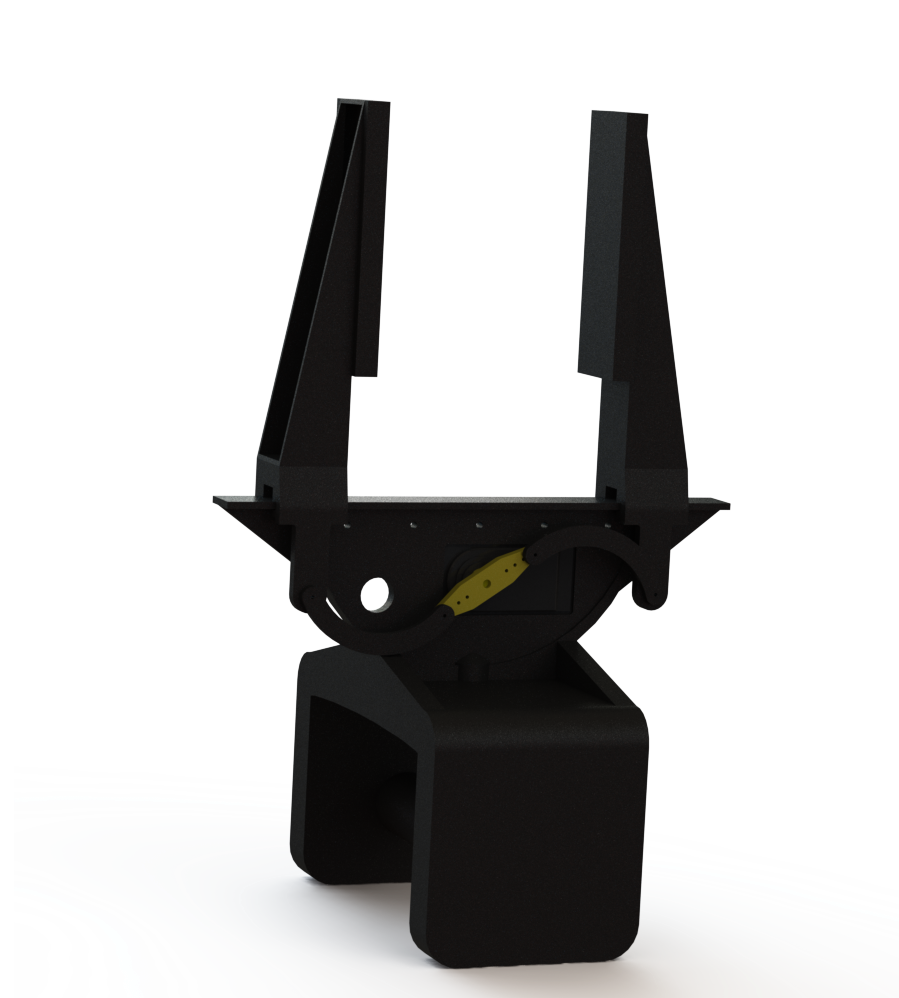
\includegraphics[width=0.25\columnwidth]{2d/3DModelsPics/o1.png}
  \label{fig:sub1}
\end{subfigure}%
\begin{subfigure}
  \centering
  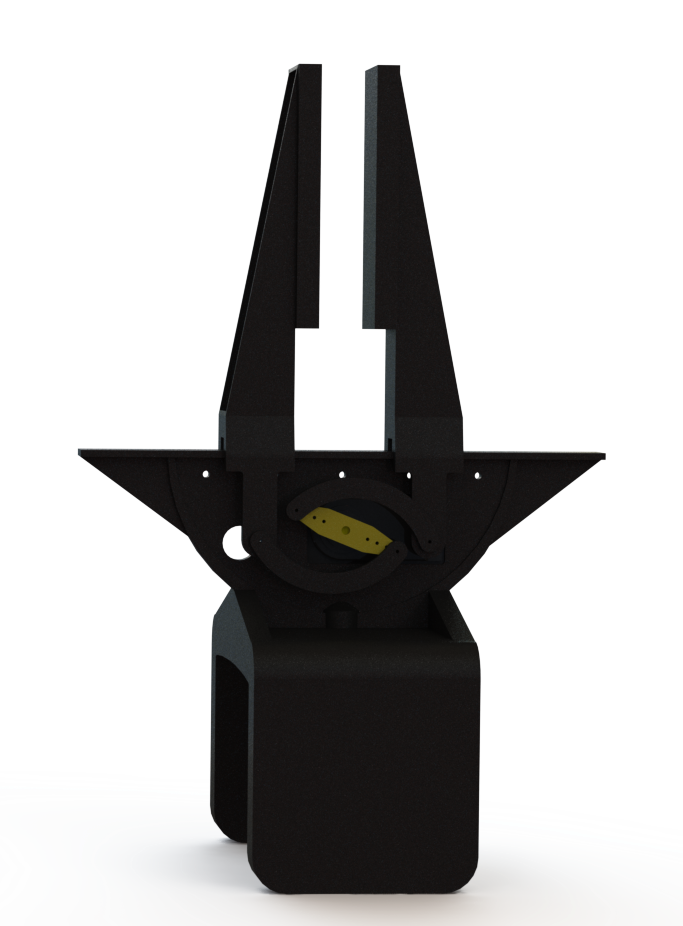
\includegraphics[width=0.20\columnwidth]{2d/3DModelsPics/o4.png}
  \label{fig:sub2}
\end{subfigure}
\begin{subfigure}
  \centering
  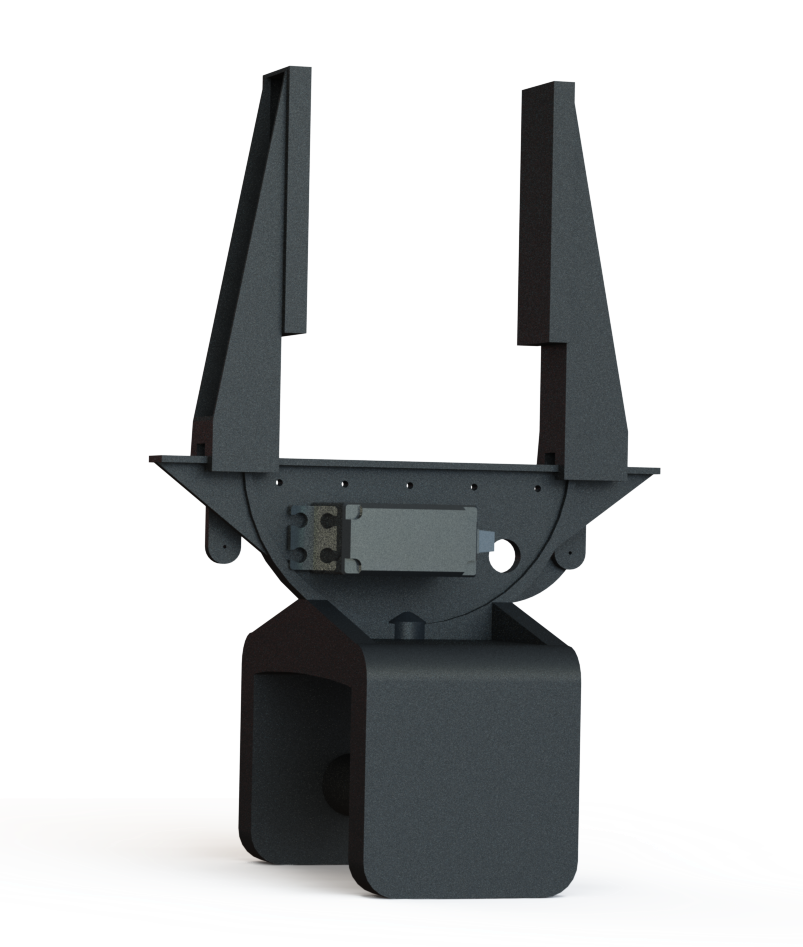
\includegraphics[width=0.235\columnwidth]{2d/3DModelsPics/o2.png}
  \begin{subfigure}
  \centering
  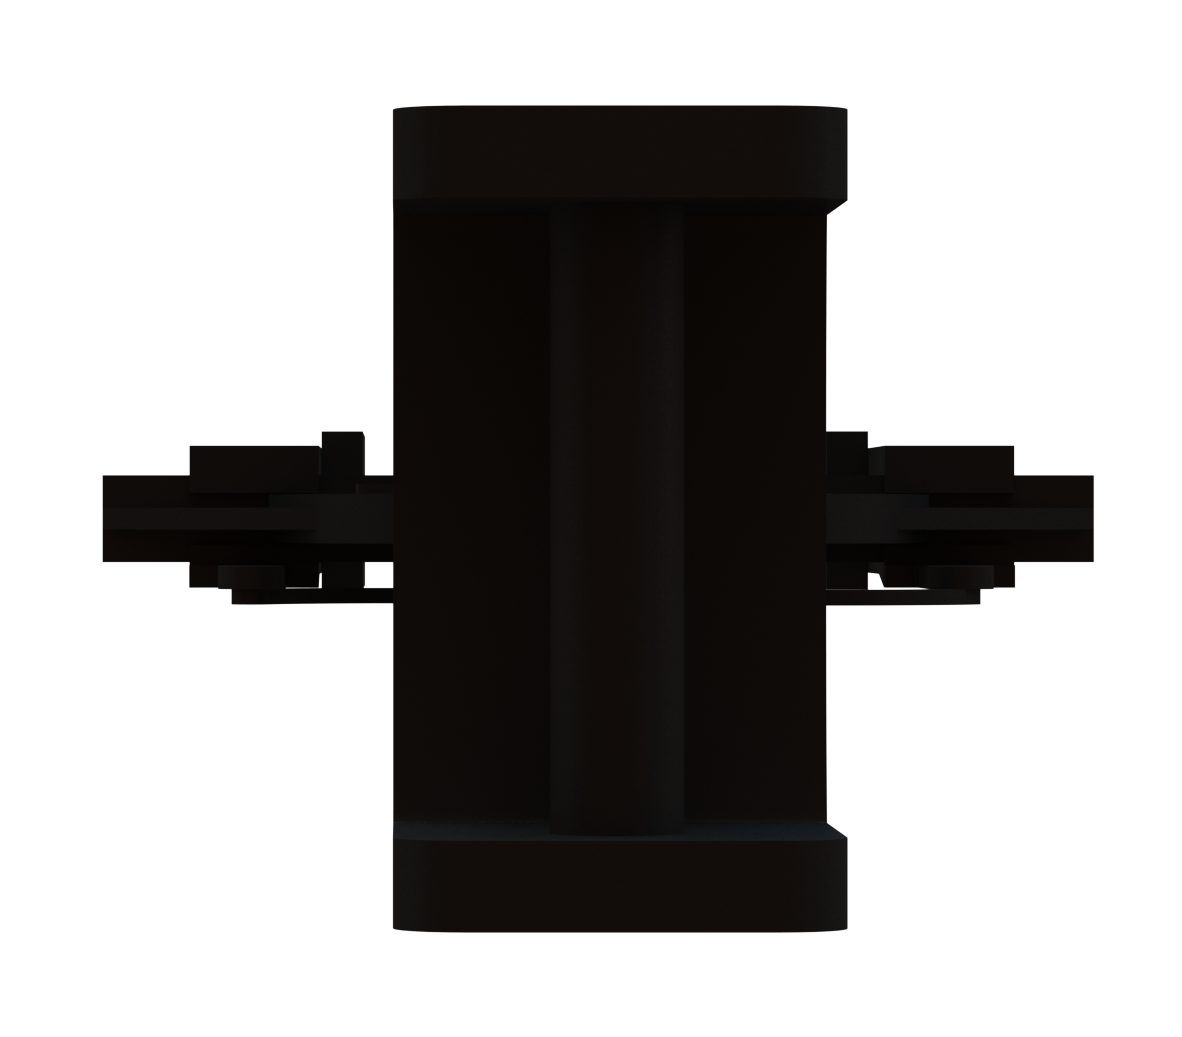
\includegraphics[width=0.17\columnwidth]{2d/3DModelsPics/o3.png}
  \label{fig:sub2}
\end{subfigure}
  \label{fig:sub2}
\end{subfigure}
\caption{SolidWorks 3D-Model Renderings of the Prototype One Assembly}
\label{fig:actual}
\end{figure}

\subsubsection{Testing \& Evaluation of Prototype One}

In order to test the model designed on SolidWorks, the first step was to utilize the Ultimaker 3D-printer accessible to our team to print a physical model out of CPE plastic. After having the components printed, the model was then assembled and prepped for testing. With the servo motor in place, our team was able to have the design opening and closing as it should based on rotational degrees of the servo motor. However, although the design assembled as anticipated, two key drawbacks went against the set of constraints and criteria stated in Tables \ref{tab:constraints} \& \ref{tab:criteria} respectively requiring the design of a second prototype. \\

The first issue that this model endured was with its general appearance. It is a criterion of this project that the model is to resemble that of a human hand. However, this prototype was designed in a way to mimic a robotic end-effector that has a negligible resemblance to a human hand. Being pitched as a prosthetic hand, this caused controversy due to its lack of human-like characteristics resulting in potential disregard by a user in need. This downfall led to the need for a second prototype addressing this concern. 

\newpage
\subsection{Mechanical Design: Prototype Two}

After the first design failed to meet the requirements of the project, a second model was designed on SolidWorks. A key drawback to the first prototype that needed to be addressed when creating the second was the aesthetic appearance of a human hand. With that said, the team sought out to create a model meeting two key points: (1) resembles a human hand with five fingers including a pinky finger, ring finger, middle finger, index finger and thumb (2) the hand should still include a single degree of freedom mechanism as done in prototype one only utilizing two fingers to grasp items. When brainstorming ideas it was also decided that this prototype would be sized in a way that the electrical hardware including a Raspberry Pi, Arduino mega, breadboard and all circuitry connecting the components would fit directly on the hand.\\

With power an issue, a new mechanical design was implemented for the second prototype. It was determined that the best way to achieve a powerful, yet controllable grip was utilizing a new servo motor and gears. To achieve this, a DS3218MG servo paired with two 1-inch diameter, 32 toothed gears were chosen. Concerning the model of the new prototype, a 5.5x6 inch palm was created such that leaving room for electrical hardware. Having a palm of such large numbers resulted in the need for fingers standing an inch thick each. The grasping mechanism was designed utilizing the index hands index finger and thumb. The thumb was strategically fixed on the underside of the palm whereas the index finger, powered by the servo motor can open and close freely on the thumb. The servo motor with a gear mounted to it has been fixed to the backside of the hand with the gear meshed to another gear fixed to a shaft mounted to the index finger. With this setup, as the motor spins, the gear transfers rotation to the second gear allowing the index finger to move in one degree of freedom. Figure \ref{fig:aa} provides a 3D rendering visual of how this design was setup. With a team member still required to hold the prosthetic during testing, the prototype was designed with a handle fixed the backside of the hand using triangular supports. The 2D drawings for prototype two can be found in Appendix A.1.2.


\begin{figure}[H]
\centering
\begin{subfigure}
  \centering
  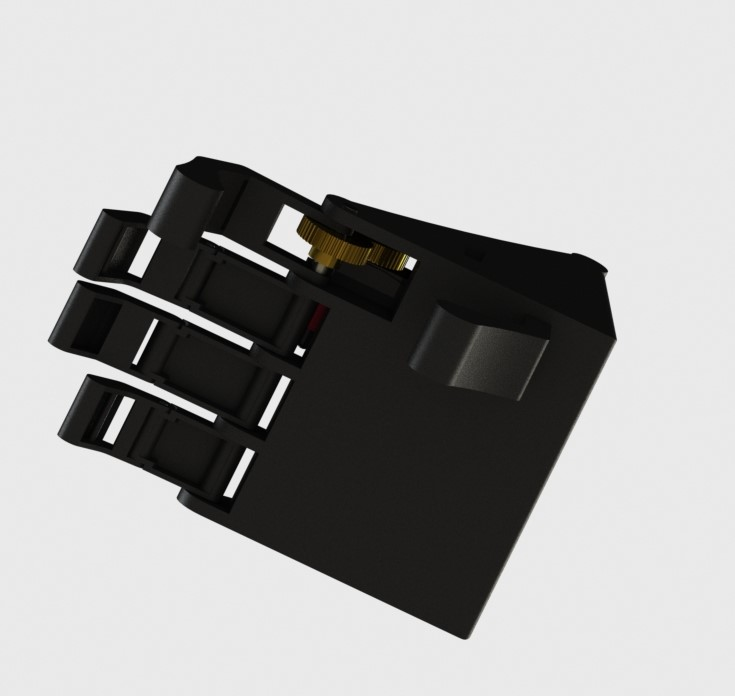
\includegraphics[width=0.28\columnwidth]{2d/3DModelsPics/m1.jpg}
  \label{fig:sub1}
\end{subfigure}%
\begin{subfigure}
  \centering
  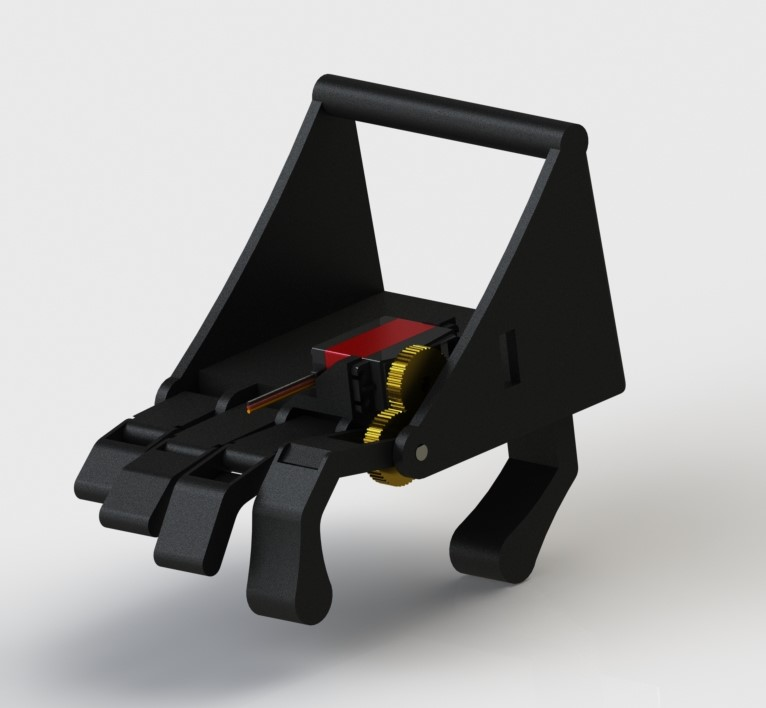
\includegraphics[width=0.287\columnwidth]{2d/3DModelsPics/m2.jpg}
  \label{fig:sub2}
\end{subfigure}
\begin{subfigure}
  \centering
  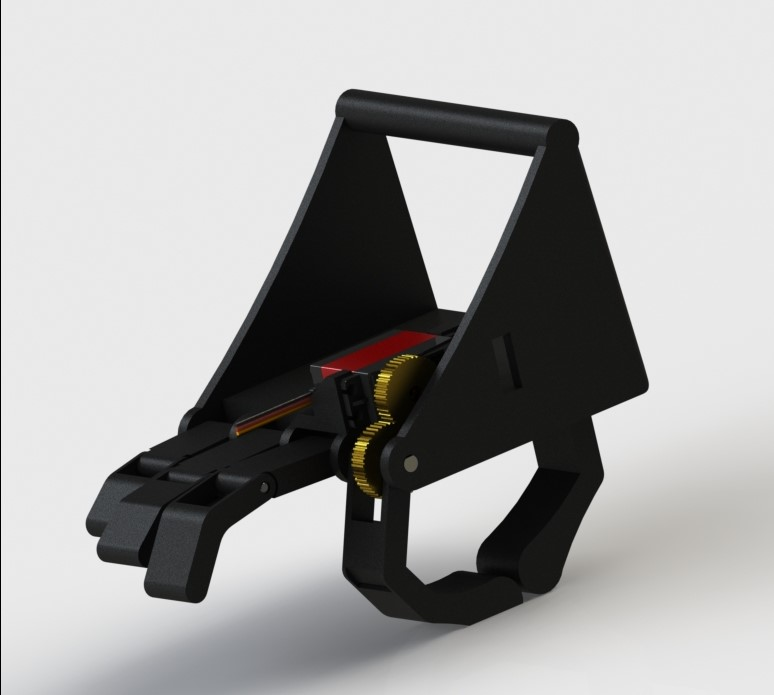
\includegraphics[width=0.295\columnwidth]{2d/3DModelsPics/m3.jpg}
  \begin{subfigure}
  \centering
  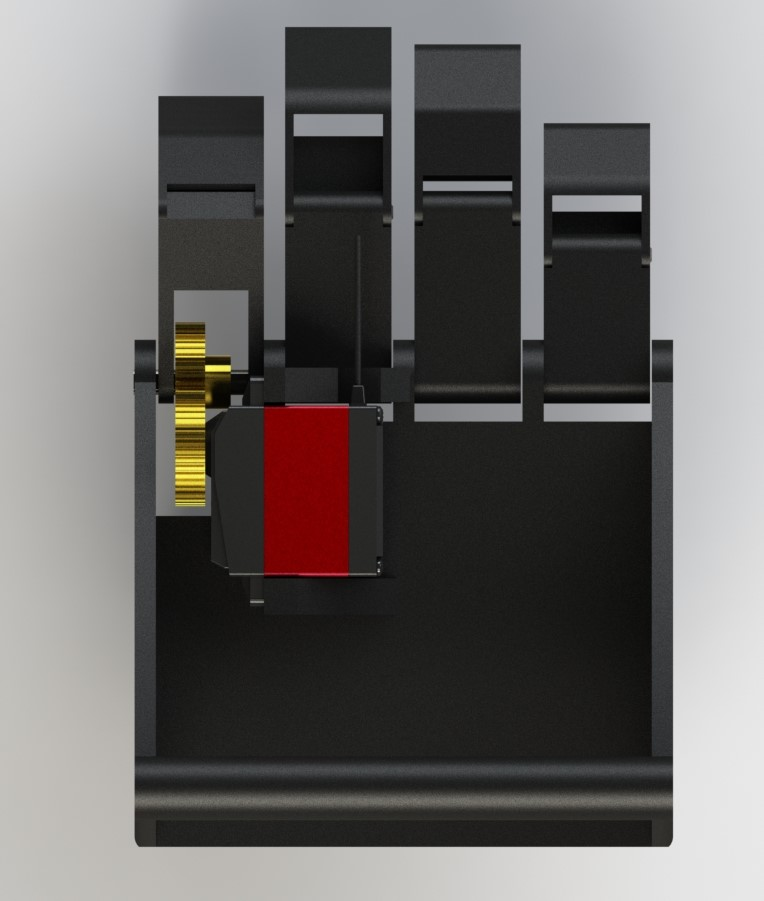
\includegraphics[width=0.26\columnwidth]{2d/3DModelsPics/m4.jpg}
  \label{fig:sub2}
\end{subfigure}
  \label{fig:sub2}
\end{subfigure}
\caption{SolidWorks 3D-Model Renderings of the Prototype Two Assembly}
\label{fig:aa}
\end{figure}

\subsubsection{Testing \& Evaluation of Prototype Two}

Although the second prototype was a large improvement aesthetically over the first, there were still ways that the design did not pass resulting in a third and final prototype. With the design of prototype two done in a way that all electrical components are to be fixed to the prosthetic, the size of the hand was compromised. This means that with the average hand width being 3.5 inches, this prototype is vastly larger with a size of 5.5 inches. With a dramatically large size paired with all circuitry mounted to the hand, the weight constraint of 0.65 kg was exceeded with prototype two violating the weight constraint. However, simply removing the electrical components hinders an unnecessarily large, aesthetically unappealing prototype.\\

In comparison to any modern hand, this prototype stands to be far too large even as a model. However, regardless of the size, although five fingers are in place, the hand's contours are very hard on the eyes. As can be seen in figure \ref{fig:aa}, the prototype has a very large bulky shape similar to that of a rectangular prism lacking basic curves and contours of a human hand. With these issues evident, it was no question that a third and final prototype was required to answer all downfalls faced by prototypes one and two.

\newpage

\subsection{Mechanical Design: Prototype Three}

The third and final design took an approach that ensured all criteria and constraints were met as well as all downfalls with prototypes one and two addressed. This final design was modeled in a way that resembled prototype two, however, correcting all issues faced. With heavy consideration, it was concluded that the best design to reduce both the weight and size of the hand is to house the electrical hardware in a location away from the hand using extended wiring. With this design in place, the only electrical component mounted to the palm is the servo motor with the gear mechanism. This allowed the physical size of the palm to reduce dramatically matching the approximate size of an average human hand. This cut the weight down to a value of 0.175kg which generously fits within the constraint of a max weight of 0.65kg. In terms of the mechanical grasping mechanism, the same thumb-index finger mounted to the pair of meshed gears was utilized from the second design. Aesthetics was strongly focused on in the final prototype. Resembling a hand is a key constraint that was achieved through heavy curvature and shaping based on that of an actual hand. In order to physically hold the model for testing, a wrist with an attached handle was designed in a way that it can be discretely screwed into the back of the palm. However, due to the COVID-19 pandemic, this component was not 3D-printed but can be seen in the 3D rendered model shown in Figure \ref{fig:actual3d}. Figure \ref{fig:actual3} displays four photos taken of the final model of the prosthetic. The 2D drawings for prototype three can be found in Appendix A.1.3. \\

\begin{figure}[H]
\centering
\begin{subfigure}
  \centering
  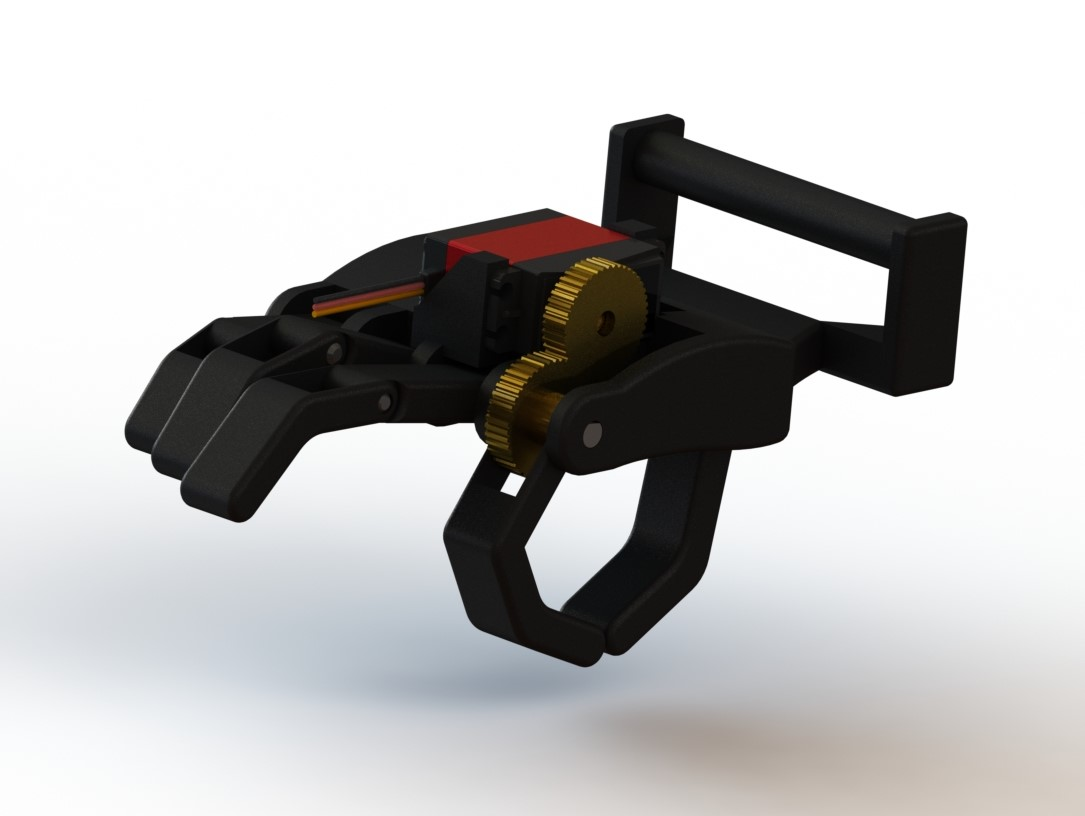
\includegraphics[width=0.25\columnwidth]{2d/3DModelsPics/n1.jpg}
  \label{fig:sub1}
\end{subfigure}%
\begin{subfigure}
  \centering
  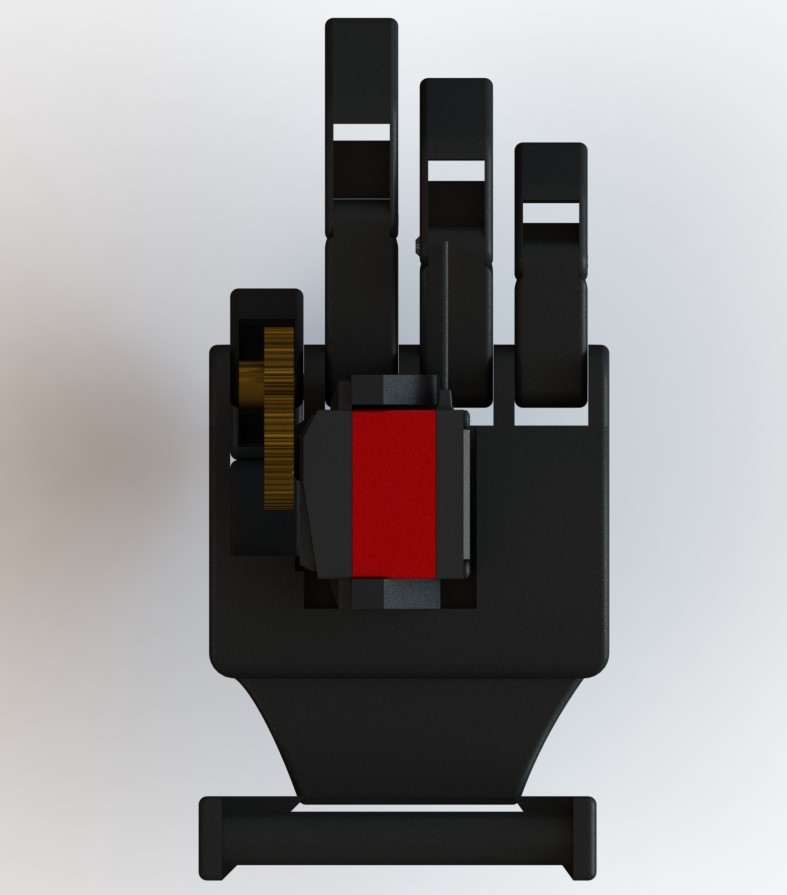
\includegraphics[width=0.20\columnwidth]{2d/3DModelsPics/n2.jpg}
  \label{fig:sub2}
\end{subfigure}
\begin{subfigure}
  \centering
  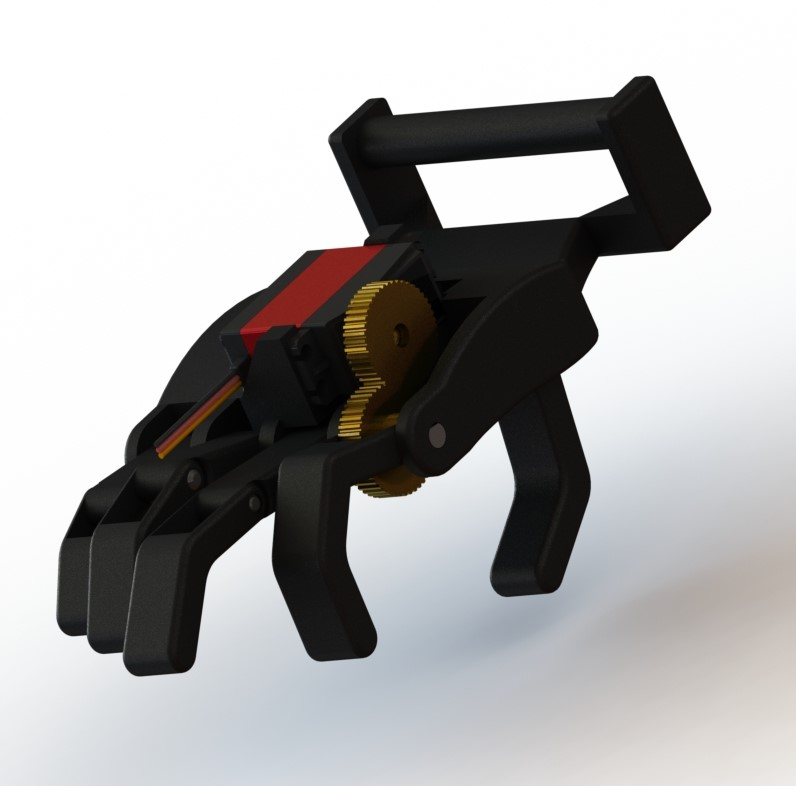
\includegraphics[width=0.235\columnwidth]{2d/3DModelsPics/n3.jpg}
  \begin{subfigure}
  \centering
  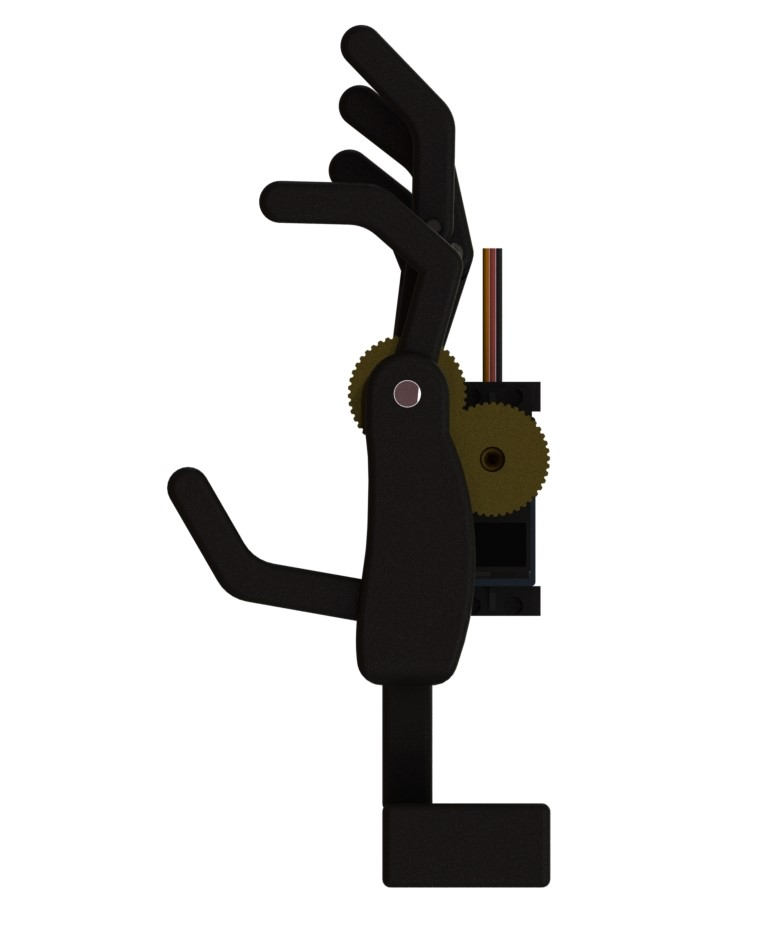
\includegraphics[width=0.18\columnwidth]{2d/3DModelsPics/n6.jpg}
  \label{fig:sub2}
\end{subfigure}
  \label{fig:sub2}
\end{subfigure}
\caption{SolidWorks 3D-Model Renderings of the Final Assembly}
\label{fig:actual3d}
\end{figure}

\begin{figure}[H]
\centering
\begin{subfigure}
  \centering
  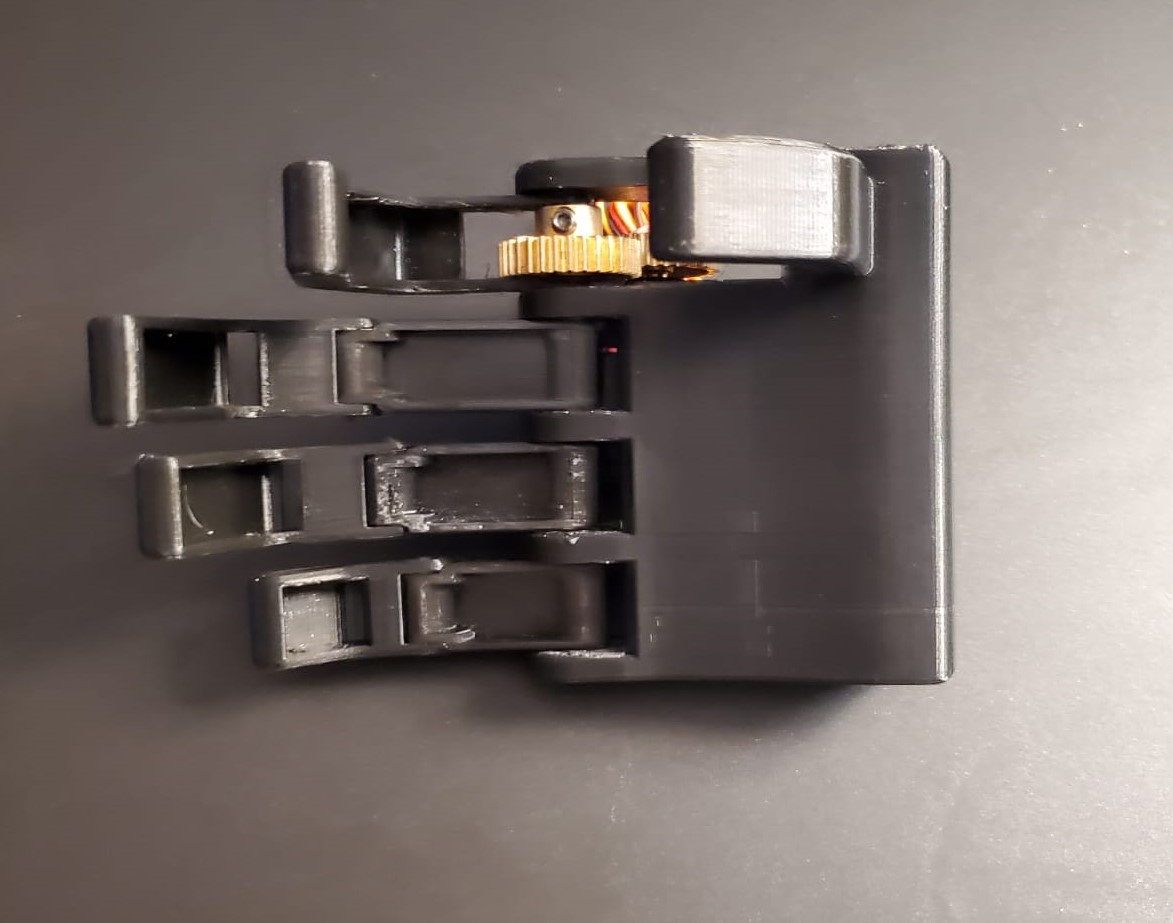
\includegraphics[width=0.25\columnwidth]{2d/1.jpeg}
  \label{fig:sub1}
\end{subfigure}%
\begin{subfigure}
  \centering
  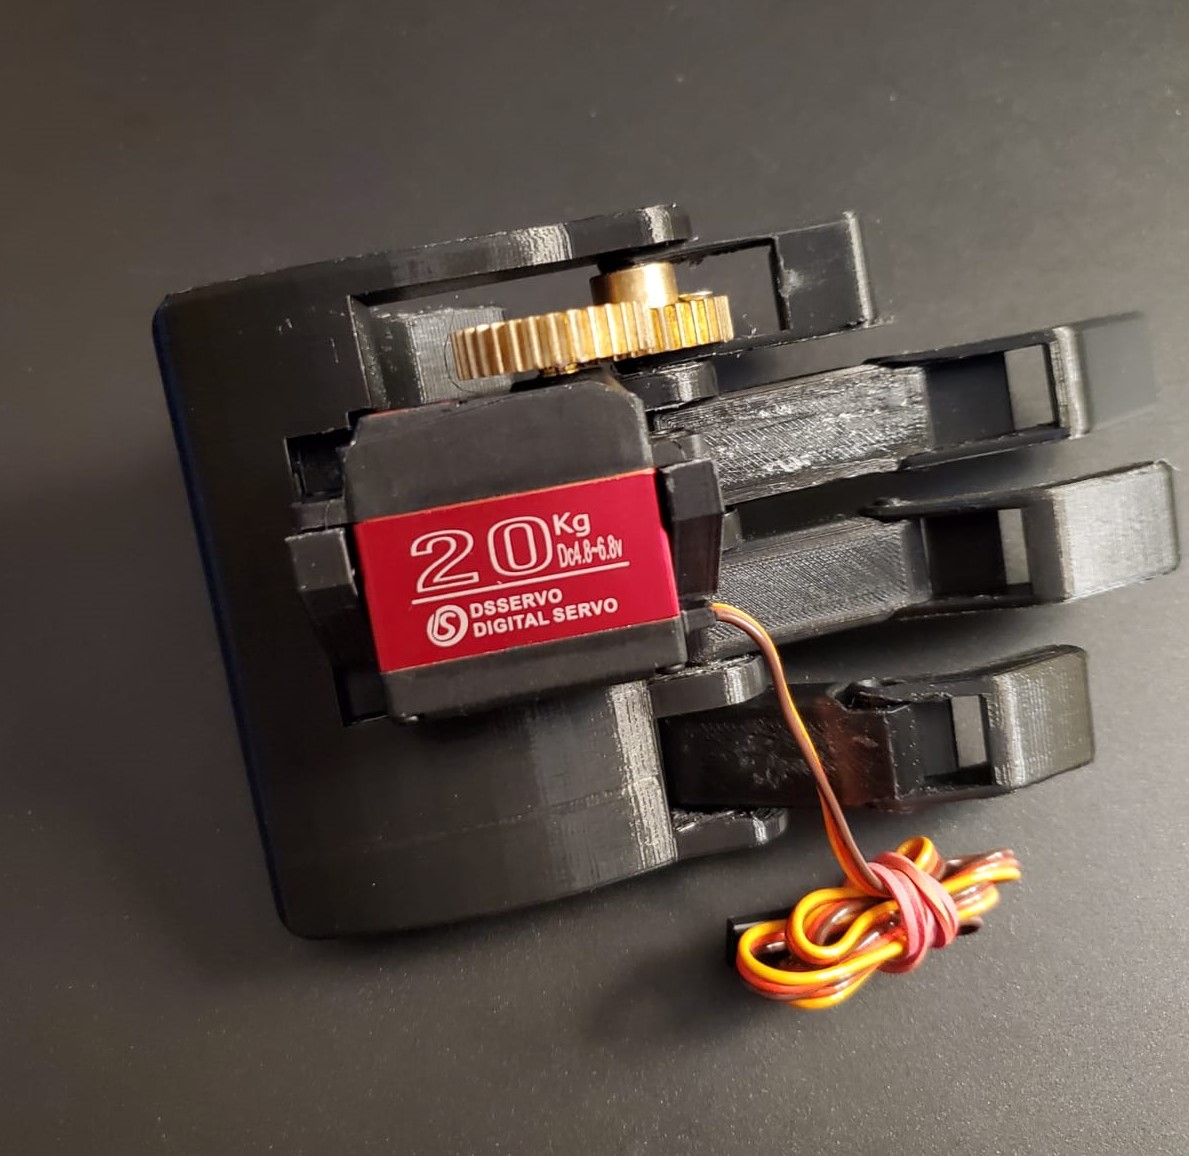
\includegraphics[width=0.20\columnwidth]{2d/2.jpeg}
  \label{fig:sub2}
\end{subfigure}
\begin{subfigure}
  \centering
  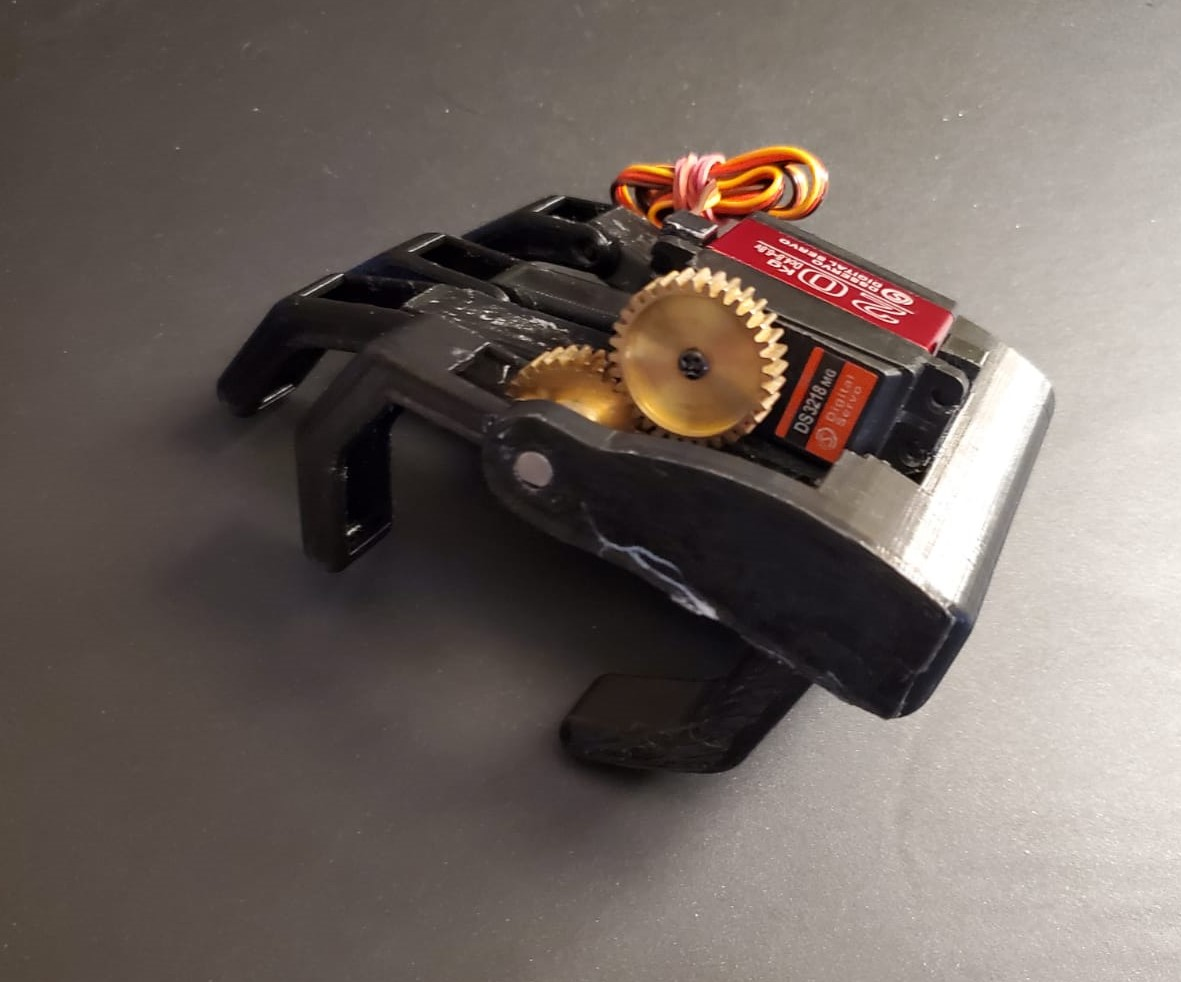
\includegraphics[width=0.235\columnwidth]{2d/3.jpeg}
  \begin{subfigure}
  \centering
  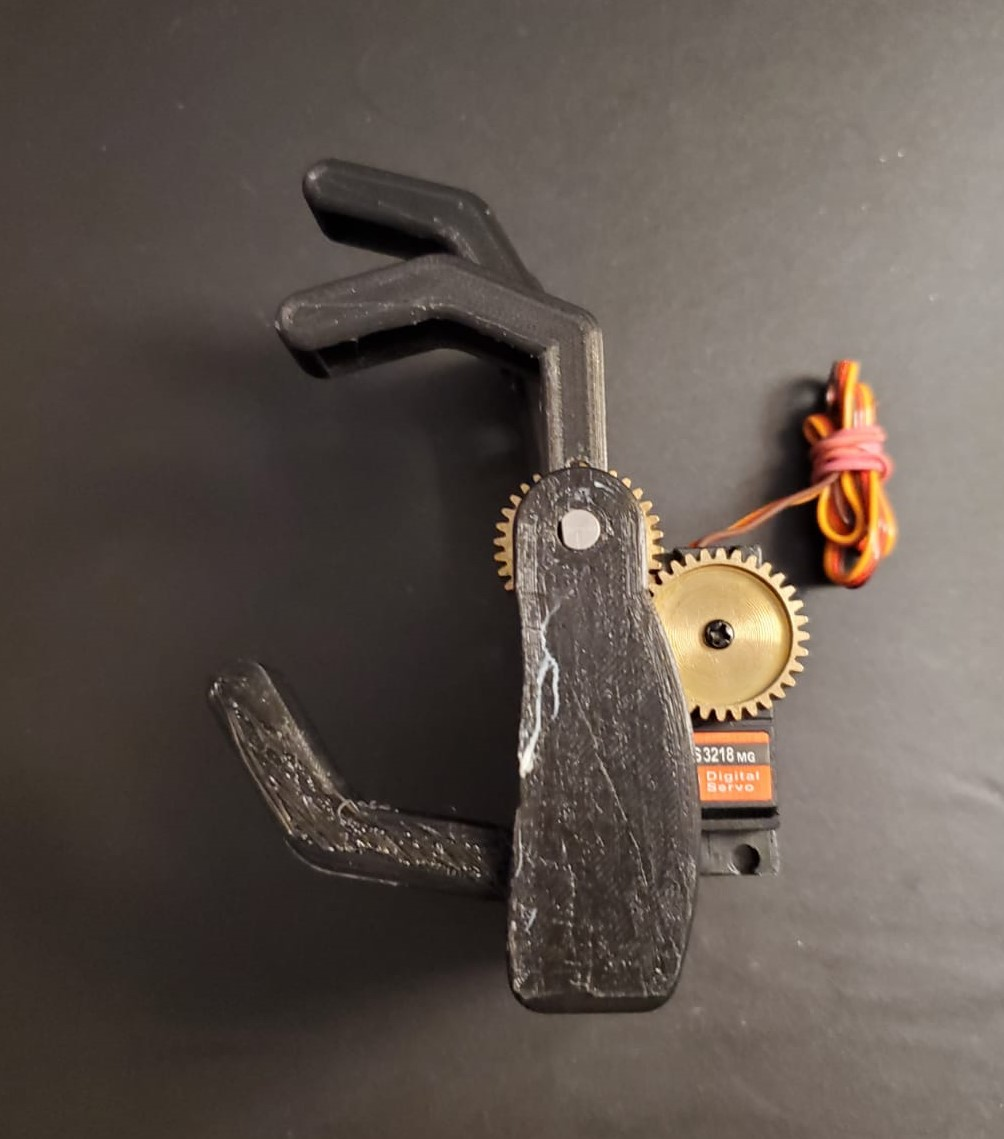
\includegraphics[width=0.17\columnwidth]{2d/4.jpeg}
  \label{fig:sub2}
\end{subfigure}
  \label{fig:sub2}
\end{subfigure}
\caption{Images of the Final 3D-Printed Model}
\label{fig:actual3}
\end{figure}

\newpage
\subsubsection{Testing \& Evaluation of Prototype Three}

When designing the third prototype it was important given the time circumstances that this model was required to meet all requirements without the need for a fourth prototype. Saying this, much thought and effort went into the final design. Concerning the mechanical structure of the project, there are three key constraints and criteria that need to be met. The first lies in the aesthetics of design, meaning, the prototype is to resemble a human hand as best as possible. Second, lies with the weight of the device. It is crucial that the weight of the model does not exceed 0.65kg as anything heavier can potentially cause discomfort hindering use of the user. Finally, a designed mechanism for grasping objects must open to a minimum span of 6 centimeters for grasping of items.\\

To test the aesthetics of the design, the 3D-printed and assembled model was exposed to groups of peers for general out of context feedback. With the curves and design lacked by the second prototype, it was said without question that prototype three was aesthetically appealing with respect to a human hand. Looking at size, the hand compared to that of the team members was quite accurate in terms of finger shape and length as well as palm length width and thickness.\\

To analyze whether the new model meets the constraint of not exceeding a total weight of 0.65kg, the servo motor was put in place with the gears and the total assembly was weighed. The model is simplified to only the prosthetic, servo and two gears compared to model two including all electrical components weighed in at a lightweight of 0.175kg.  However, due to the COVID-19 pandemic, the wrist/handle attachment seen in Figure \ref{fig:actual3d} was not 3D-printed. With this said, the hand should weigh in slightly higher however not nearly enough to reach the maximum weight constraint.\\ 

The final constraint relating to the grasping mechanisms opening span is set such that it opens to a minimum of 6cm. The third prototype when assembled not only achieved this minimum value but instead surpassed it. Opened to its maximum realistic span prototype threes maximum span is 8cm surpassing the constraint by 2cm.\\

Having met all the required constraints and criteria in place for this project, it is without question that the third prototype was the final prototype required for this project. With flaws in the first two prototypes, the third was required to meet all requirements as the need for an additional design would have delayed the project resulting in an incomplete finish. For this reason, the third iteration was designed in such a way that no drawbacks were plausible.

\newpage

\section{Cost Evaluation}
\subsection{Required Tools and Resources}

The cost evaluation of the design will be based on the final prototype including all the components required to build the prosthetic hand. The required tools and resources, along with their description can be seen in Table \ref{tab:Des}.


\begin{table}[H]
    \centering
    \caption{Descriptions of each component}
    \vspace{3mm}
    \begin{tabular}{|l|l|}
    \hline
      & \\
    \multicolumn{1}{|c|}{Component}  & \multicolumn{1}{c|}{Description} \\ 
     & \\ \hline
     
      & \\
        CPE Filament &  The prototype of the prosthetic hand is 3D printed with black-colored \\  & copolyester (CPE) plastic. CPE is a durable and chemical-resistant material \\ & making it ideal for the prototype.  \\
        & \\ \hline 
        
         & \\
        Raspberry Pi 3 Model B & The Raspberry Pi is the central computational device used in the design. \\ & It hosts machine learning and allows for user interaction.\\ 
        & \\ \hline
        
         & \\
        Raspberry Pi Camera & The camera provides a visual component by identifying and classifying \\ & the label of the objects in front of the prosthetic hand.\\ 
        & \\ \hline
        
         & \\
        Arduino Mega 2560 & The Arduino is a microcontroller that processes sensor input and \\ & produces and output signal to the Raspberry Pi.\\ 
        & \\ \hline
        
         & \\
        Tactile Sensor & The sensors allow the fingers to determine the force applied to an object.\\ 
        & \\ \hline
        
         & \\
        20kg DS3218MG Servo Motor &  The servo motor is used to control the movement of the gears on the \\ &  prosthetic hand. Therein facilitating the movement of the finger.\\ 
        & \\ \hline
        
         & \\
        Breadboard jumper wires & The jumper wires connect all the electrical components in the design.\\ 
        & \\ \hline
        
         & \\
        Gear & The gears translate motor torque to finger movement. \\ 
        & \\ \hline
    \end{tabular}
    \label{tab:Des}
\end{table}

3D printed components should essentially last a lifetime, however, with daily use, it will start to wear out over time. It is estimated that the prosthetic hand will only have to be replaced once in the users lifetime as it is made from a very strong and durable CPE plastic. Having to only replace the prosthetic once makes it a very cost-effective product. In section 4.2 below holds the projects bill of materials. It can be seen that the cost for one hand is approximately \$316.00 making it relatively cheap compared to others. With a simplified design, the replacement of individual components is an easy yet inexpensive task. \\

\newpage
\subsection{Bill of Materials}

The bill of materials for the prototype can be seen in Table \ref{tab:BOM}. It includes the specific components, the quantity, cost per unit and total costs. It is determined that the final cost of one prototype is about \$316.00. As mentioned previously, current prosthetic hands in the market can cost thousands of dollars and is not as cost-effective as our prosthetic hand. The team's prosthetic hand requires minimal resources and tools and is comprised of inexpensive components.\\




\begin{table}[H]
    \centering
    \caption{Bill of Materials for the prosthetic hand}
    \vspace{3mm}
    \begin{tabular}{cccc}
    \hline
         Component & Quantity & Cost per Unit & Total Cost \\
         \hline
            CPE Filament & 1.5 Roll & - & \$110\\\\
            Raspberry Pi 3 Model 3 & 1 & \$48.00 & \$48.00\\\\
            Gear & 2 & \$24.00 & \$48.00\\\\
            Arduino Mega 2560 & 1 & \$40.00 & \$40.00\\\\
            Raspberry Pi Camera & 1 & \$30.00 & \$30.00\\\\
            Tactile Sensor & 2 & \$10.00 & \$20.00\\\\
            20kg DS3218MG Servo Motor & 1 & \$16.00 & \$16.00\\\\
            Breadboard jumper wires & 10 & \$0.40 & \$4.00\\\\
            TOTAL COST & - & -  & \$316.00\\\\
    \hline
    \end{tabular}
    \label{tab:BOM}
\end{table}

\newpage

\section{Conclusion and Recommendations}
Although the project was not finished due to COVID-19, the project was completed to the best of the teams ability. The team was able to design and create the final prototype of the prosthetic hand, however testing and training the model was not performed. The deep learning algorithm was conceptualized, but it was not pragmatically implemented. As mentioned previously, \emph{Calandra et al.} proposed an end-to-end action-conditional model that learns re-grasping policies from raw visuotactile data. Their deep, multimodal CNN predicts the outcome of a candidate grasp adjustment as a Markov decision process and executes a grasp by iteratively selecting the most promising actions. We primarily drew insights from this work to approximate our results if the project were fully completed. \emph{Calandra et al.} completed 6,450 grasping trials from over 65 training objects and further augmented this data to over 18,000 data points. Using K-fold (K=3) cross-validation, they were able to achieve an accuracy of 80.28\% ± 0.68\%. Without action as an input, as in the case of our model, they achieved an accuracy of 76.43\% ± 0.42\%. Notable differences between our work include the use of tactile sensors that output numerical data instead of an image, approach angle being determined by the user, MLP for the optical input instead of a CNN, and a continuous feedback control strategy. Therefore, we hope to see a higher accuracy when applied to our hand. \\

As with any project, there is always room for improvements and future works. Due to the circumstances, the algorithm was not complete and therefore the algorithm could be extended to ensure all components are operating according to the project scope. This means the algorithm will be able to perform object classification with the use of the camera and attempting to grasp the object, meanwhile dynamically classifying the rigidity based on peripheral sensory feedback with the tactile sensors. Testing of the final prototype was also not completed, and with this said, future work post-pandemic would be to train/test the model. The prototype could be redesigned, allowing for testing on amputees and/or people with birth defects, in need of a prosthetic. At this point, components of the prototype were chosen based on availability in the Robotics Institute lab. Therefore, minimizing the size and weight of all components including tactile sensors, servo motors, and all computational hardware would be ideal for a commercial product. In the current state, a battery bank used to charge portable devices is being used to power the electrical hardware. Battery banks are quite heavy resulting in discomfort for a user. To eliminate this issue, the implementation of a Lithium-Polymer battery similar to that of a smartphone should be used. Being a non recyclable material, the used Copolyester (CPE) plastic filament used for the model should be swapped with a more environmentally friendly alternative such that of Lactic Acid (PLA) plastic. As a single degree of freedom device, the ability to grasp objects is limited. Future works would be to design a multi-degree of freedom prototype, including the use of all five fingers for grasping resulting in a more human-like functionality. 


\newpage
\bibliographystyle{unsrt}  
\bibliography{references}

\newpage
\pagenumbering{arabic}% resets `page` counter to 1
\renewcommand*{\thepage}{A\arabic{page}}
\appendix 

\section{Appendix}

\subsection{2D Drawings}
\subsubsection{Design One}
\begin{figure}[H]
    \centering
    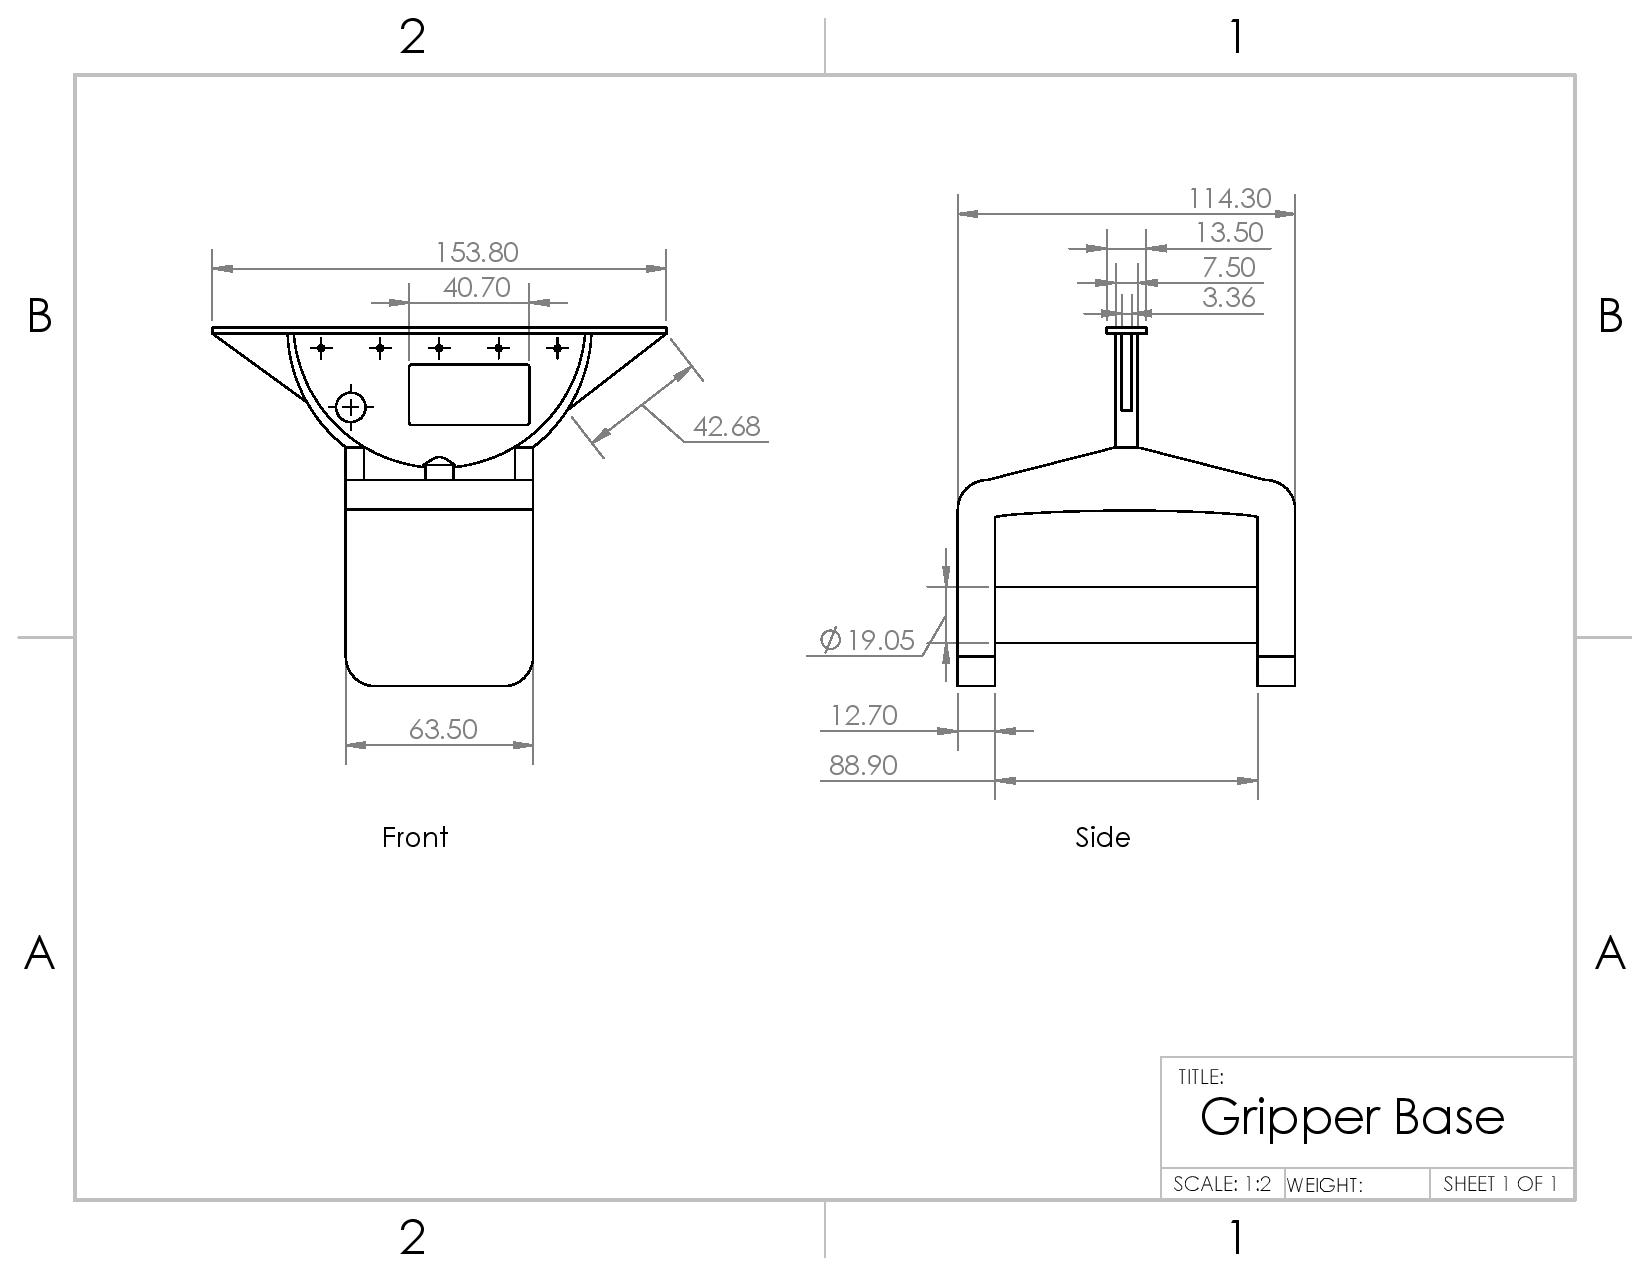
\includegraphics[width=0.75\columnwidth]{2d/Base-page-001.jpg}
    \caption{2D Drawing of Gripper Base}
    \label{RLDiagram}
\end{figure}
\begin{figure}[H]
    \centering
    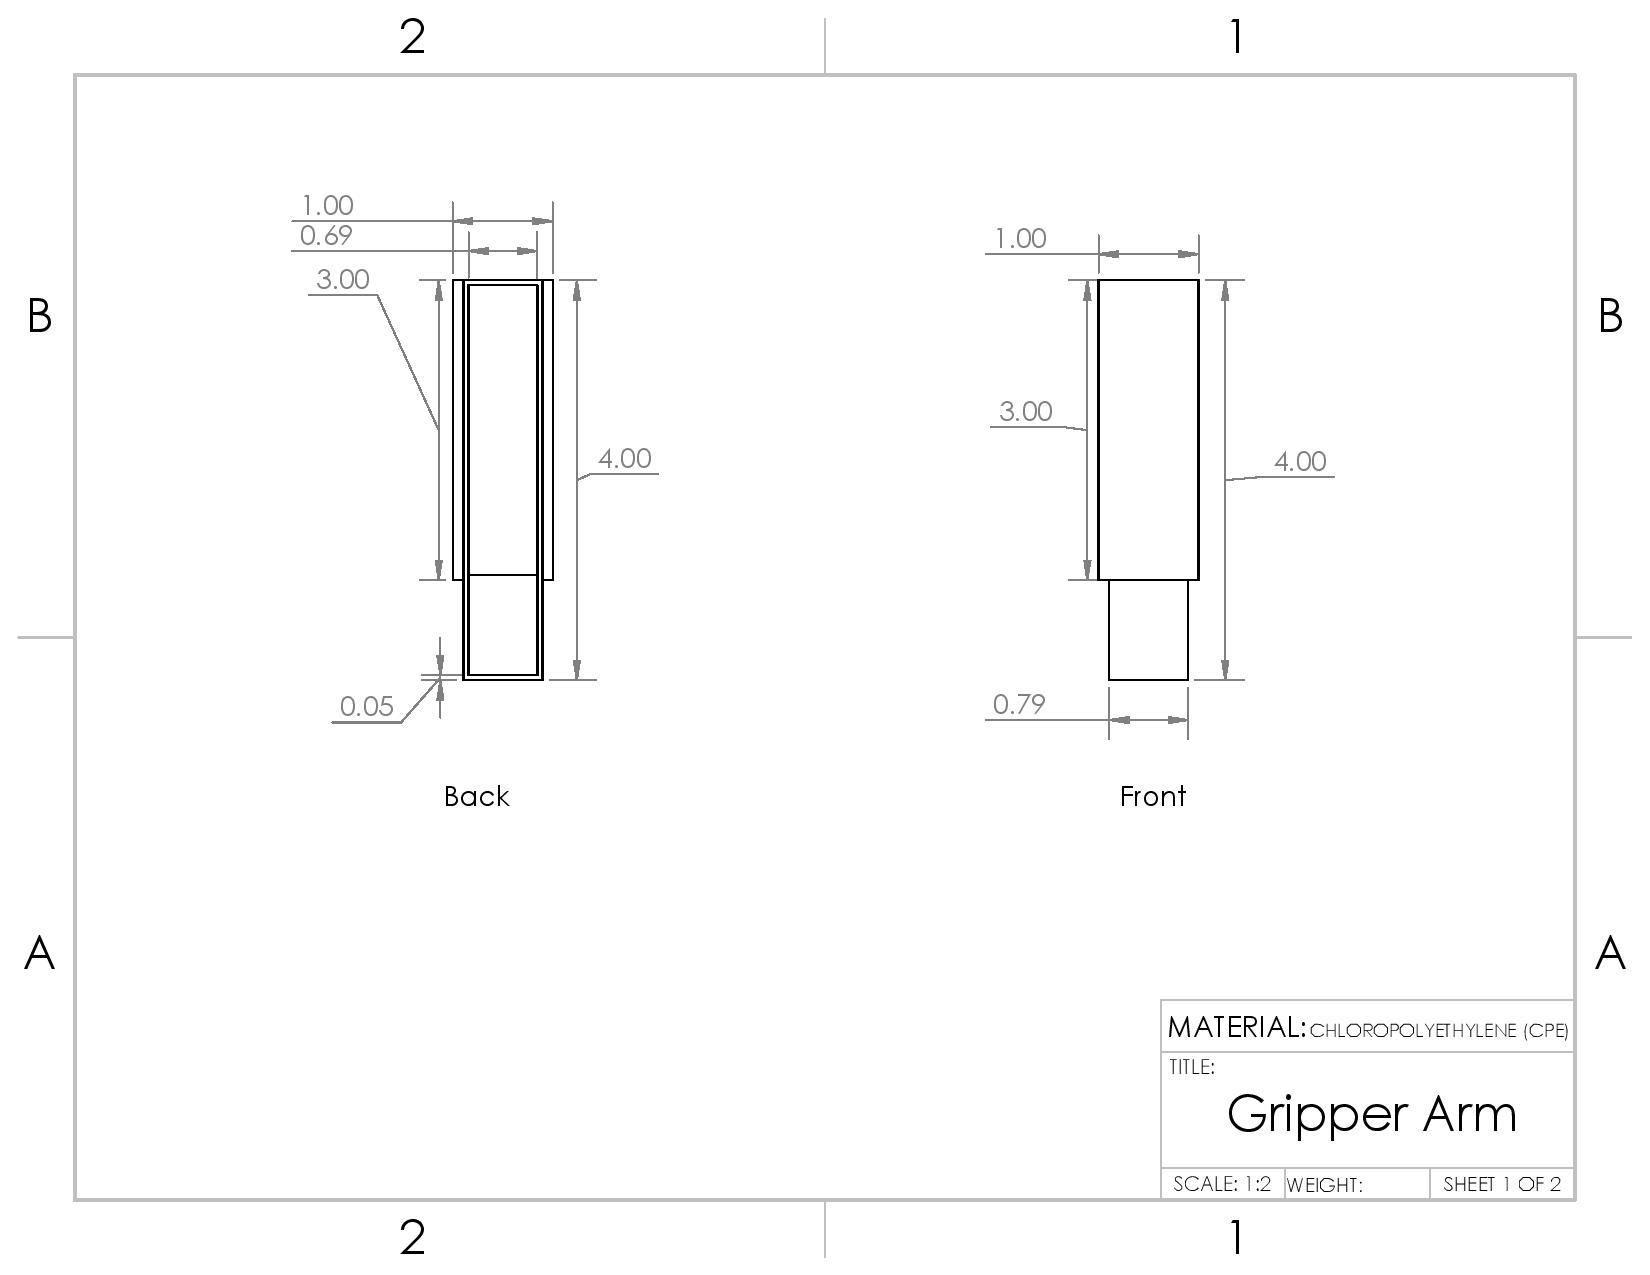
\includegraphics[width=0.75\columnwidth]{2d/Arm-page-001.jpg}
    \caption{2D Drawing of Gripper Arm: : Back View and Front View}
    \label{RLDiagram}
\end{figure}
\begin{figure}[H]
    \centering
    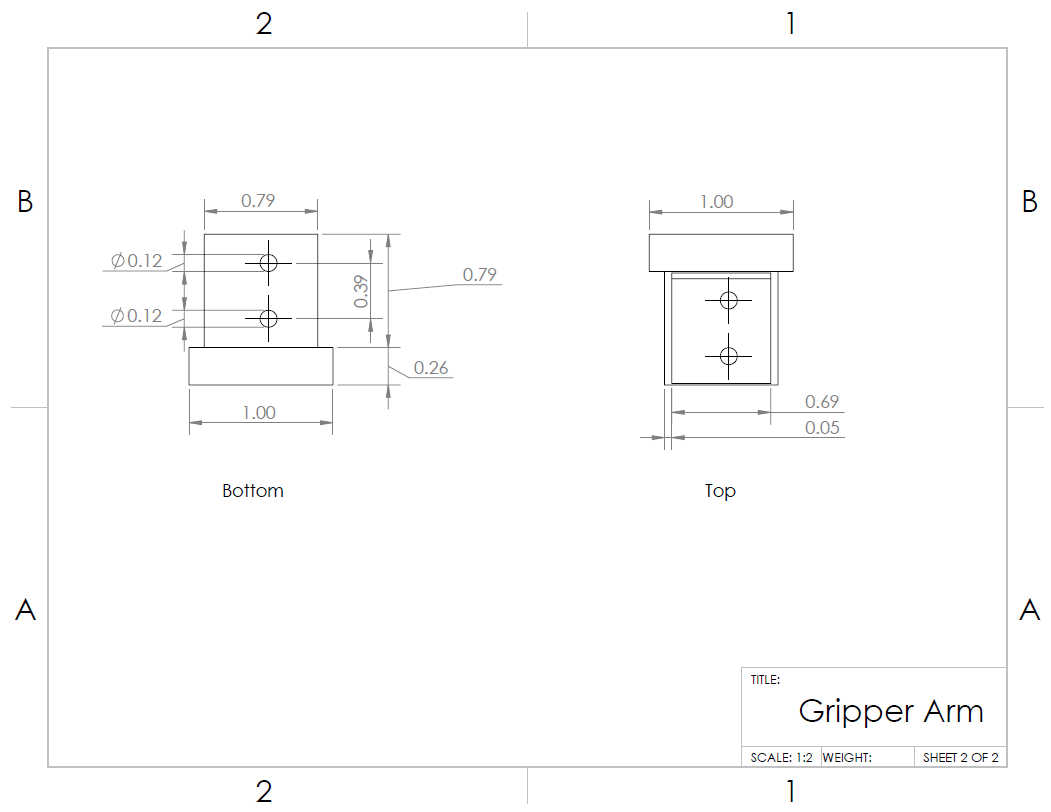
\includegraphics[width=0.75\columnwidth]{2d/Screenshot (53).png}
    \caption{2D Drawing of Gripper Arm: Top View and Bottom View}
    \label{RLDiagram}
\end{figure}
\begin{figure}[H]
    \centering
    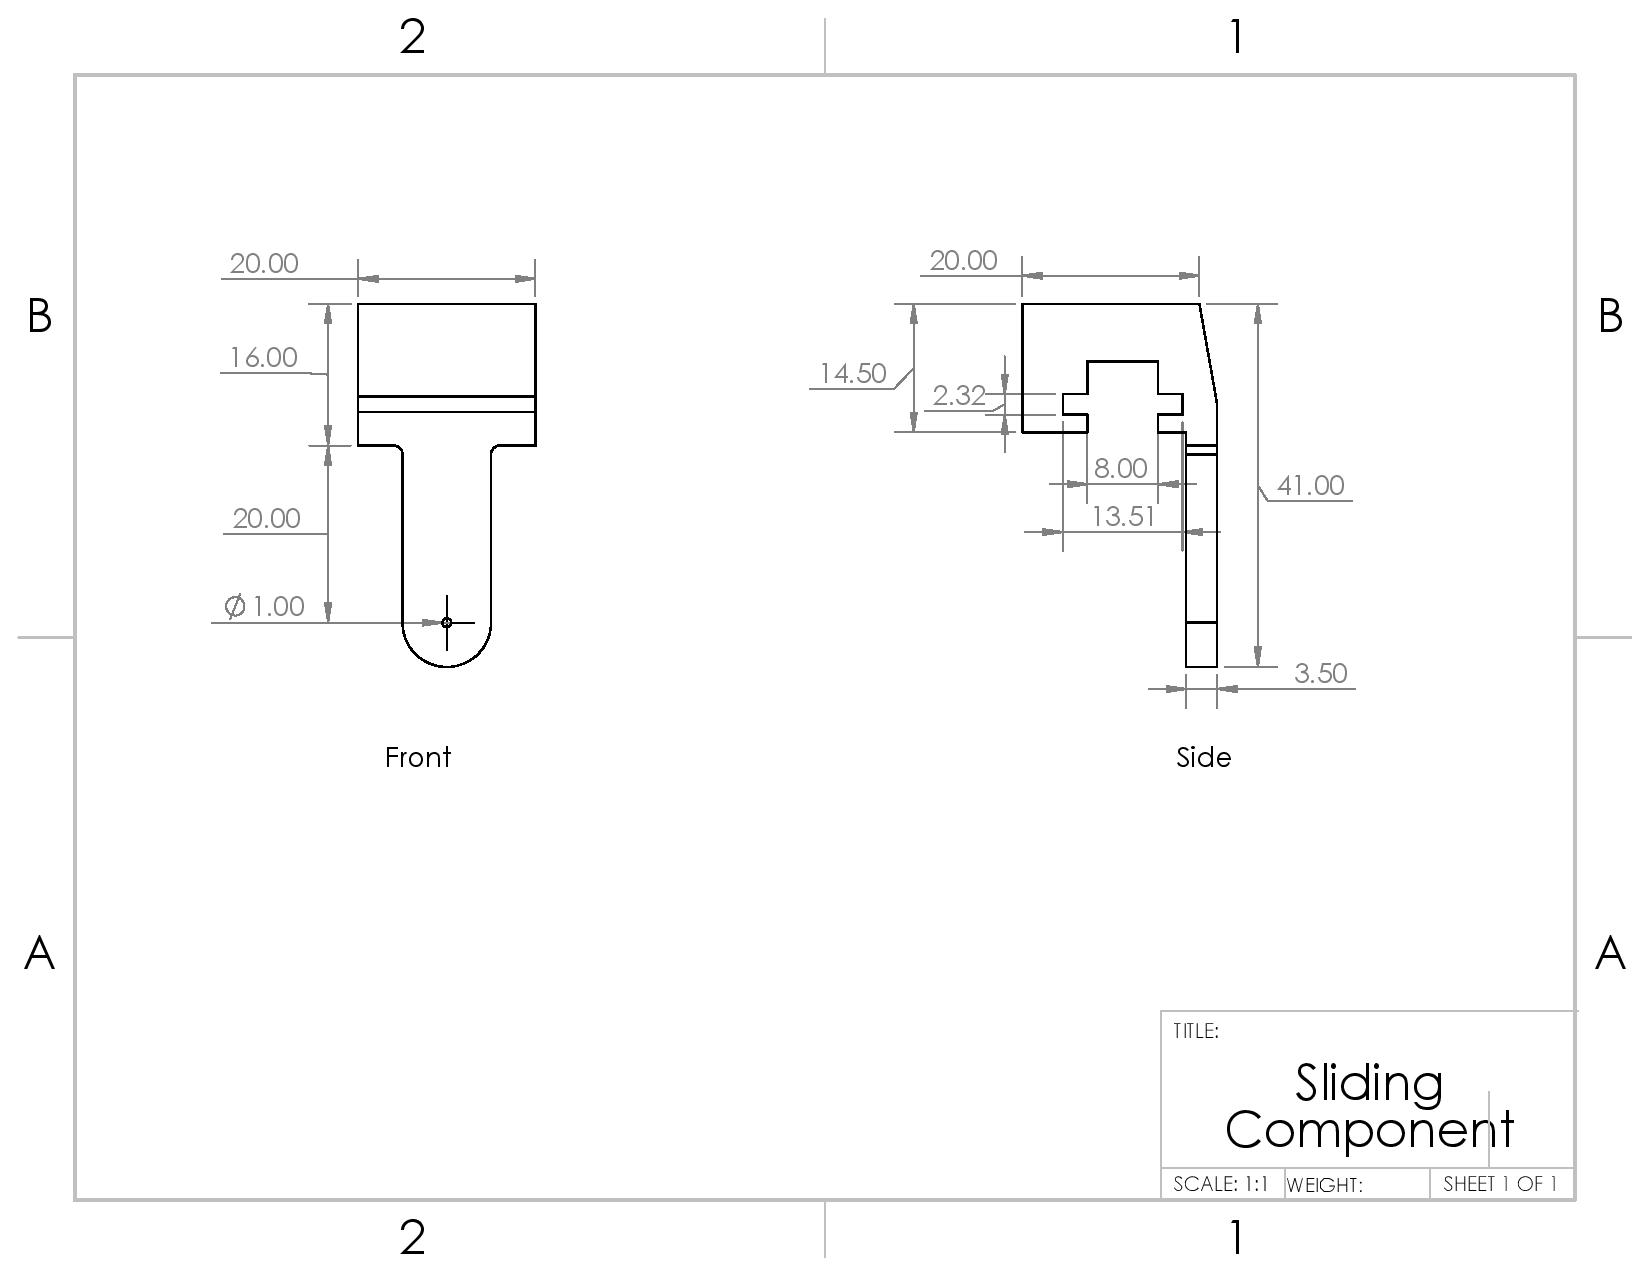
\includegraphics[width=0.75\columnwidth]{2d/Sliding component-page-001.jpg}
    \caption{2D Drawing of Gripper Slider}
    \label{RLDiagram}
\end{figure}
\begin{figure}[H]
    \centering
    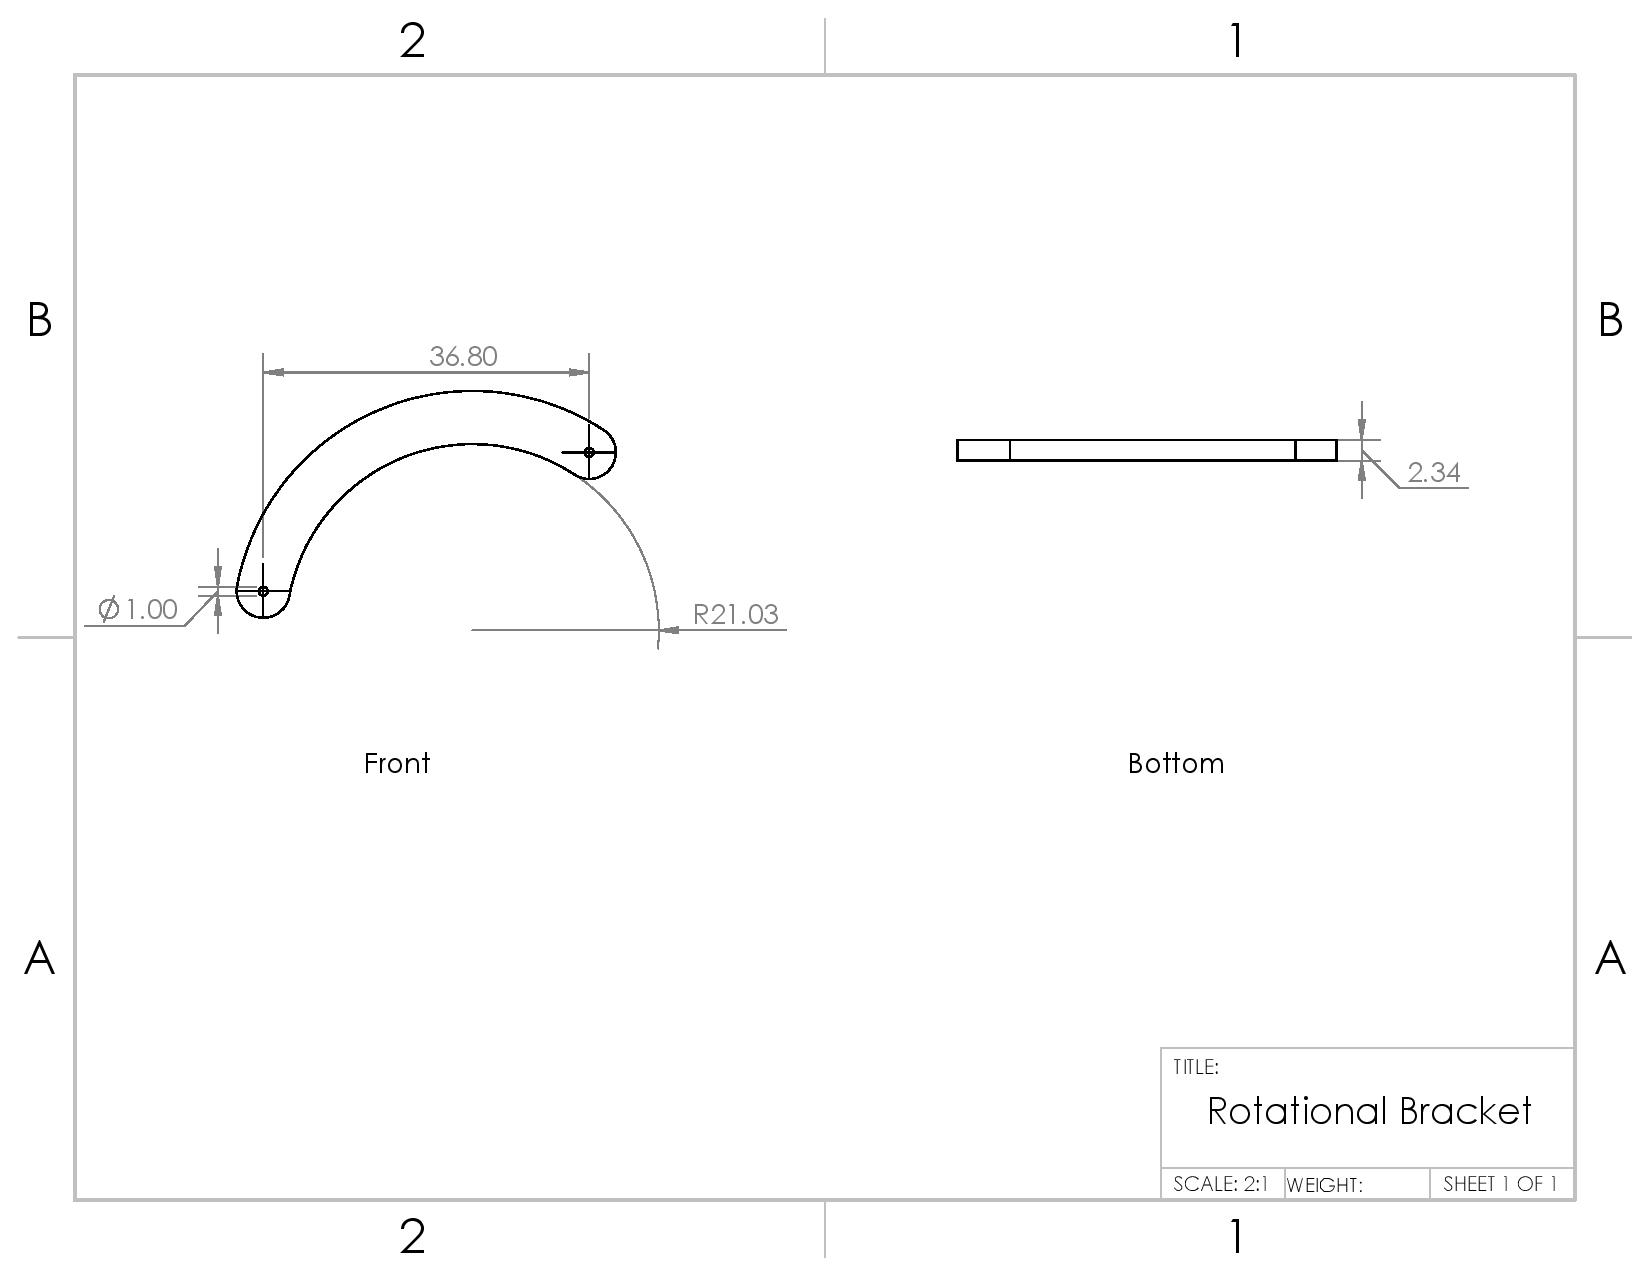
\includegraphics[width=0.75\columnwidth]{2d/swing-page-001.jpg}
    \caption{2D Drawing of Gripper Bracket}
    \label{RLDiagram}
\end{figure}

\subsubsection{Design Two}

\begin{figure}[H]
    \centering
    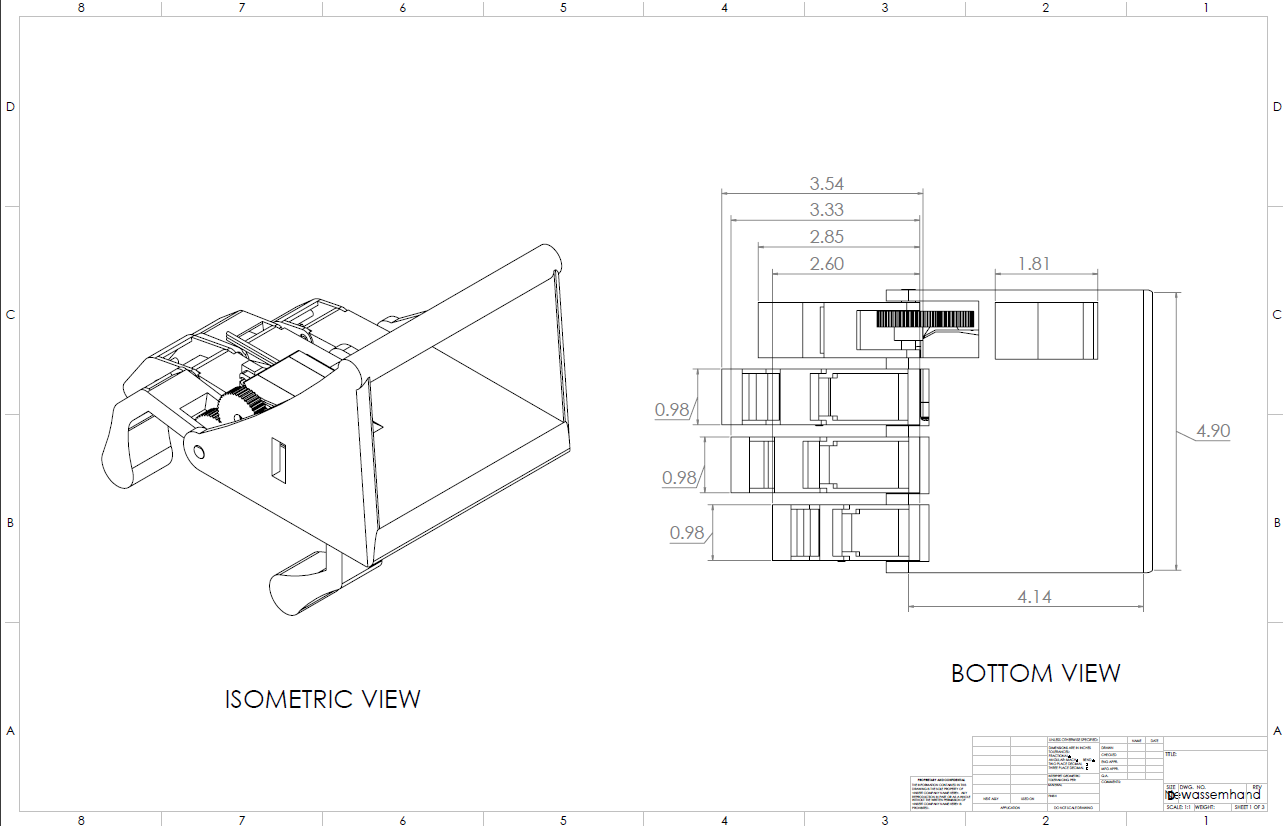
\includegraphics[width=0.75\columnwidth]{2d/3DModelsPics/Screenshot (26).png}
    \caption{2D Drawing of Prototype Two: Isometric View and Bottom View}
    \label{RLDiagram}
\end{figure}
\begin{figure}[H]
    \centering
    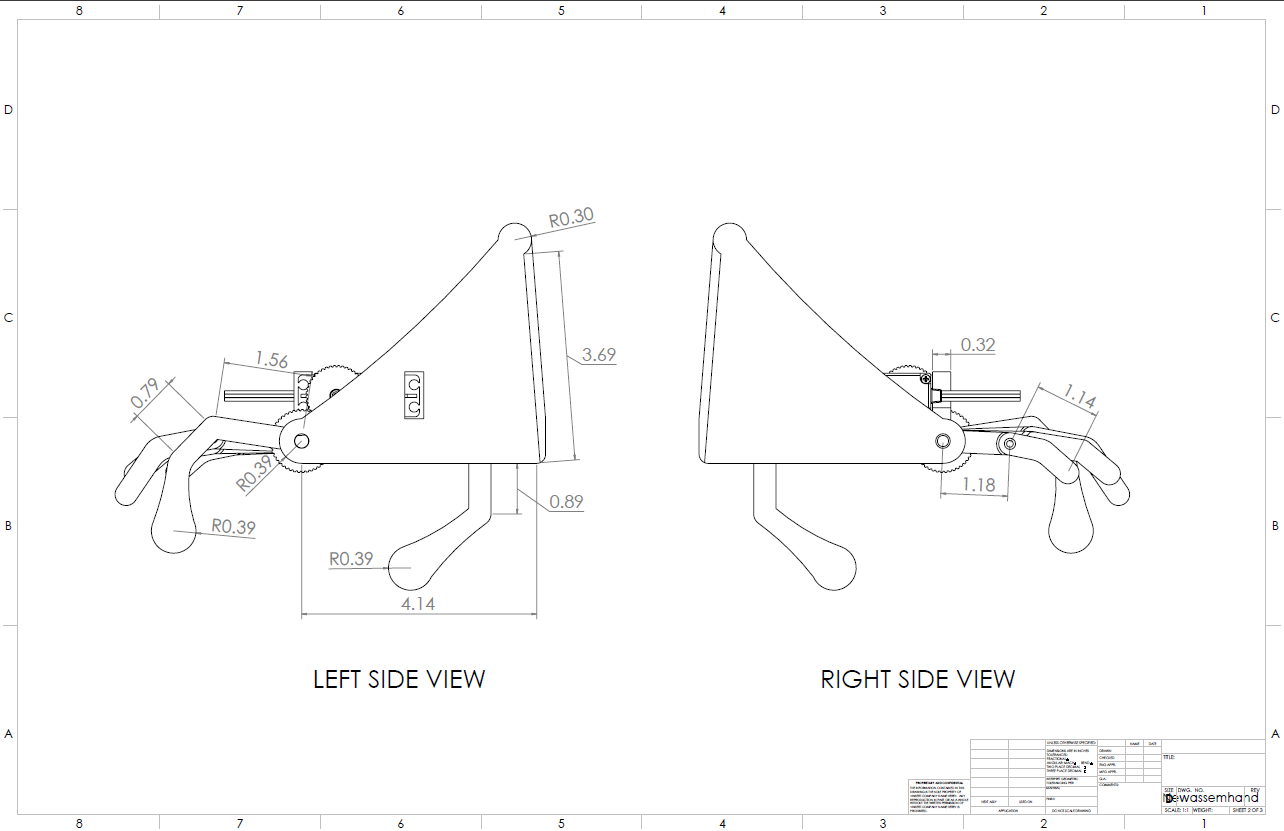
\includegraphics[width=0.75\columnwidth]{2d/3DModelsPics/Screenshot (27).png}
    \caption{2D Drawing of Prototype Two Side Views}
    \label{RLDiagram}
\end{figure}
\begin{figure}[H]
    \centering
    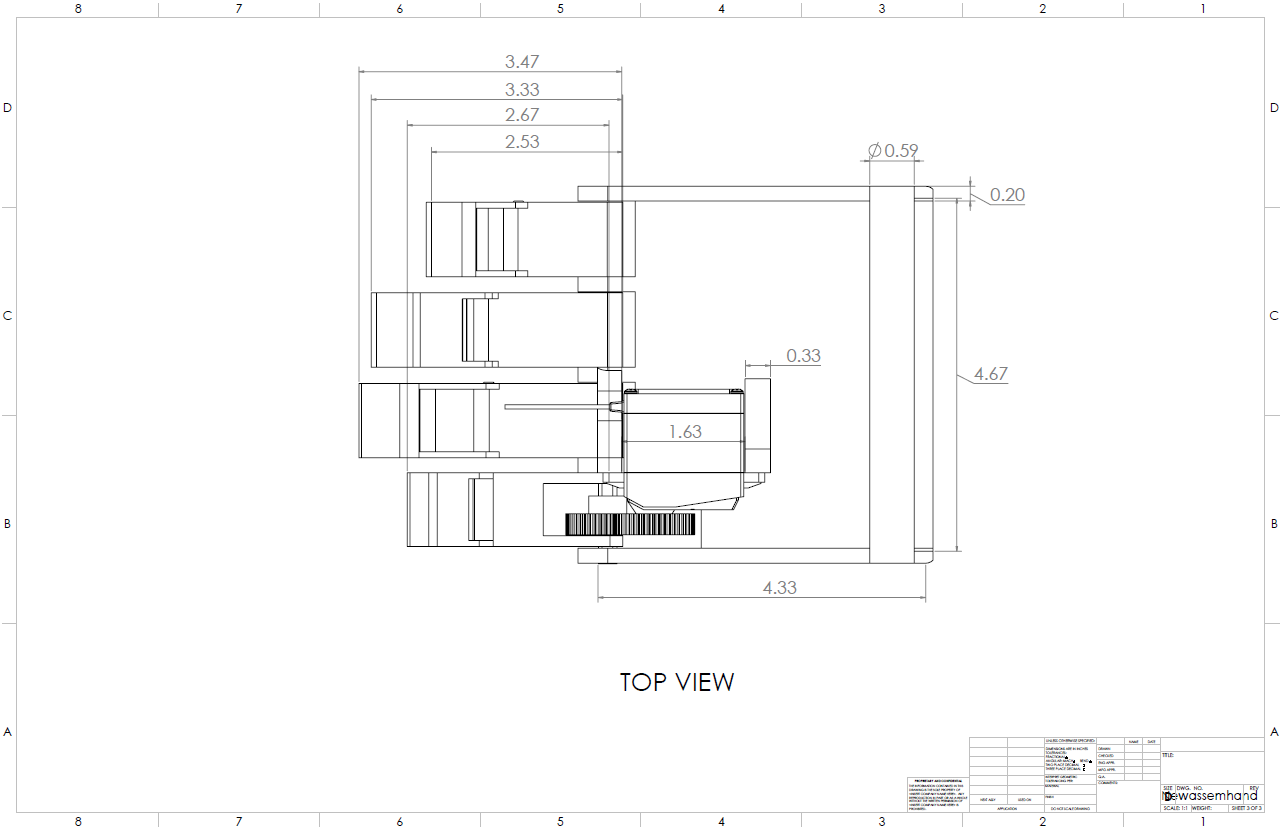
\includegraphics[width=0.75\columnwidth]{2d/3DModelsPics/Screenshot (28).png}
    \caption{2D Drawing of Prototype Two Top View}
    \label{RLDiagram}
\end{figure}

\newpage

\subsubsection{Final Design}

\begin{figure}[H]
    \centering
    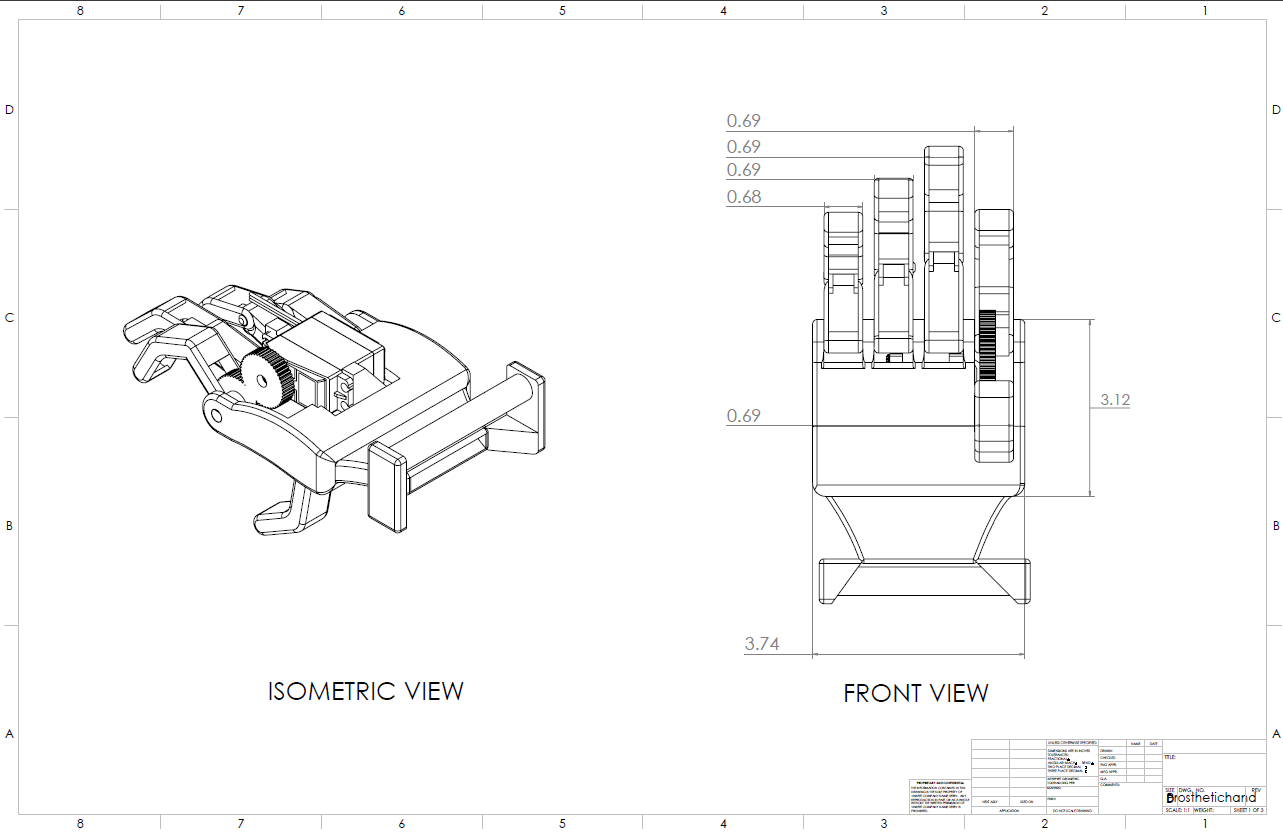
\includegraphics[width=0.75\columnwidth]{2d/3DModelsPics/Screenshot (23).png}
    \caption{2D Drawing of Prototype Three: Isometric View and Front View}
    \label{RLDiagram}
\end{figure}
\begin{figure}[H]
    \centering
    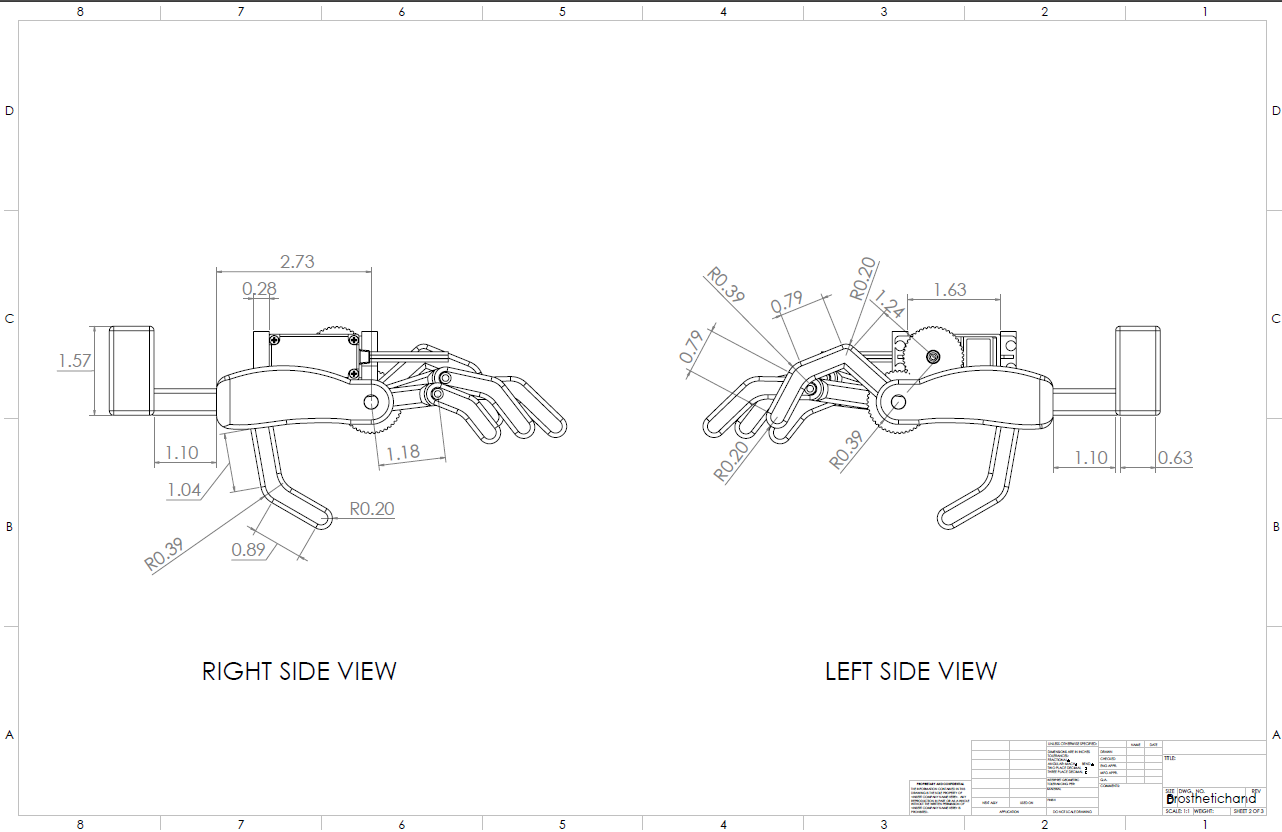
\includegraphics[width=0.75\columnwidth]{2d/3DModelsPics/Screenshot (24).png}
    \caption{2D Drawing of Prototype Three Side Views}
    \label{RLDiagram}
\end{figure}
\begin{figure}[H]
    \centering
    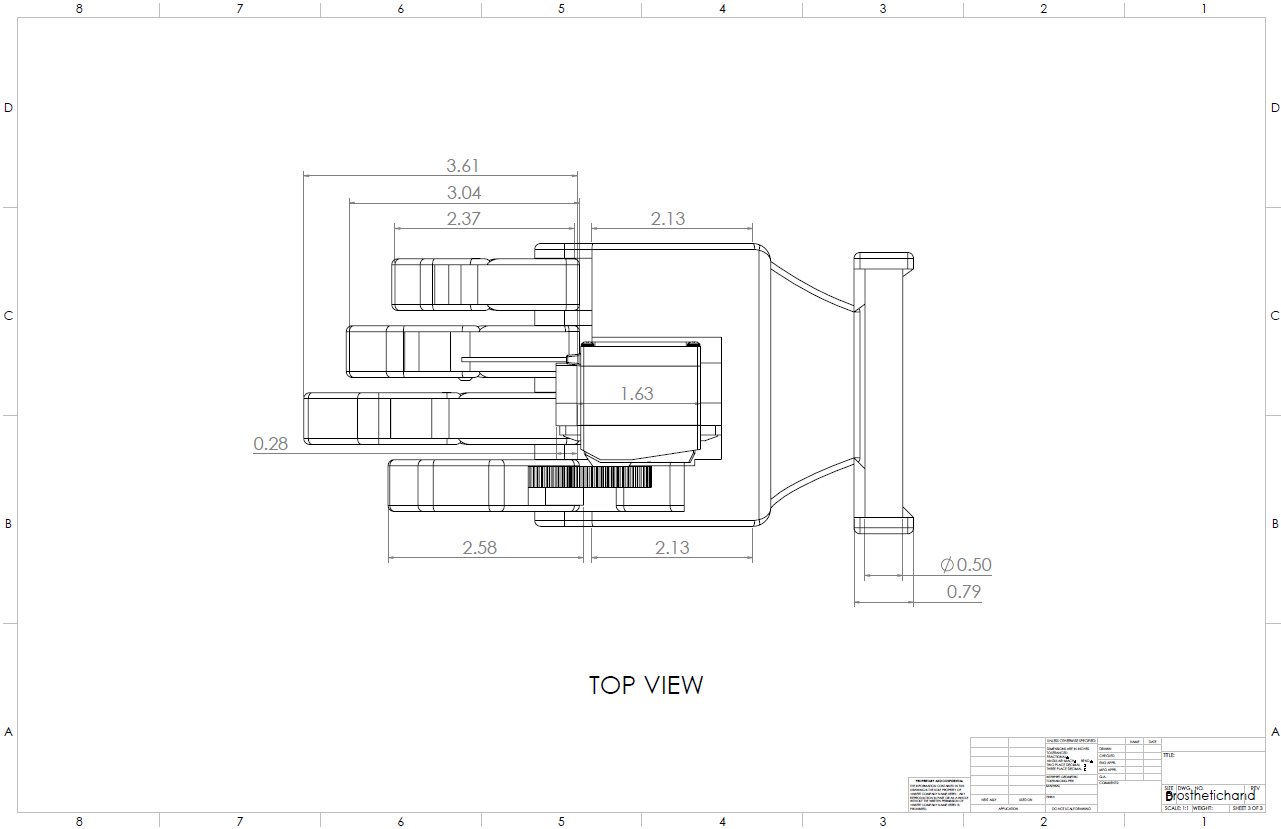
\includegraphics[width=0.75\columnwidth]{2d/3DModelsPics/Screenshot (25).png}
    \caption{2D Drawing of Prototype Three Top View}
    \label{RLDiagram}
\end{figure}


\newpage

\pagebreak

\end{document}